% How accurate LIGHT_Kr v0_2 is: the pure-krypton model, scored against
% pure-krypton measurements, with its propagated uncertainty, its
% reference point and its checks. No number here is typed by hand except
% the measurements, which carry their sources. They come from
%   overview_v0_2_numbers.tex     make_overview_v0_2.py     (\wg)
%   system_map_v0_2_numbers.tex   make_system_map_v0_2.py   (\wm)
% Build from LIGHT_Kr/docs:
%   python3 make_system_map_v0_2.py && python3 make_overview_v0_2.py
%   latexmk -pdf accuracy_overview_v0_2.tex
\documentclass[11pt]{article}
\usepackage[a4paper,margin=2.2cm]{geometry}
\usepackage[T1]{fontenc}
\usepackage[scaled=0.95]{helvet}
\renewcommand{\familydefault}{\sfdefault}
\usepackage{amsmath,amssymb}
\usepackage{sansmath}
\usepackage{booktabs,tabularx,array}
\usepackage{xcolor}
\usepackage{float}
\usepackage{enumitem}
\usepackage{graphicx}
\usepackage{tikz}
\usepackage{pgfplots}
\pgfplotsset{compat=1.18}
\usetikzlibrary{arrows.meta,decorations.pathmorphing}
\setlist{nosep, leftmargin=1.2em}
\setlength{\parindent}{0pt}
\setlength{\parskip}{5pt}
\definecolor{ink}{HTML}{0B0B0B}
\definecolor{ink2}{HTML}{52514E}
\definecolor{cE}{HTML}{2A78D6}
\definecolor{cX}{HTML}{EDA100}
\definecolor{cP}{HTML}{C46A00}
\definecolor{cV}{HTML}{A63A83}
\definecolor{cH}{HTML}{E34948}
\definecolor{cI}{HTML}{52514E}
\renewcommand{\topfraction}{0.95}
\renewcommand{\textfraction}{0.03}

% LIGHT_Kr v0_2 map numbers. GENERATED by make_system_map_v0_2.py
% from the model (0.2.0-kr). Do not edit. Rerun the script instead.
\providecommand\wmdef[2]{\expandafter\def\csname wm@#1\endcsname{#2}}
\wmdef{e.P}{100.0}
\wmdef{e.pen}{2.7}
\wmdef{e.pen2}{0.0}
\wmdef{e.G1}{20.5}
\wmdef{e.C1}{0.8}
\wmdef{e.HM}{0.0}
\wmdef{e.C2}{0.0}
\wmdef{e.76}{77.6}
\wmdef{e.stepS}{0.0}
\wmdef{e.stepP}{0.0}
\wmdef{e.G6}{2.6}
\wmdef{e.dU}{0.0}
\wmdef{e.cap}{1.1}
\wmdef{G1.krs}{20.2}
\wmdef{G1.heat}{0.3}
\wmdef{C1.kr}{0.8}
\wmdef{C1.heat}{0.0}
\wmdef{HM.ion}{0.0}
\wmdef{HM.heat}{0.0}
\wmdef{kpp.back}{5.8}
\wmdef{KPS.heat}{77.8}
\wmdef{PRAD.hv}{0.6}
\wmdef{PRAD.heat}{0.0}
\wmdef{kpp.stepP}{0.0}
\wmdef{kpp.left}{0.0}
\wmdef{krs.G2}{9.0}
\wmdef{krs.AK8}{16.9}
\wmdef{krs.stepS}{0.0}
\wmdef{krs.left}{0.0}
\wmdef{G2.ion}{6.4}
\wmdef{C2.ion}{0.0}
\wmdef{stepS.ion}{0.0}
\wmdef{stepP.ion}{0.0}
\wmdef{AK8.heat}{1.2}
\wmdef{k2s.RAD}{15.5}
\wmdef{k2s.pen}{0.0}
\wmdef{k2s.left}{0.2}
\wmdef{RAD.hv}{14.2}
\wmdef{RAD.heat}{1.3}
\wmdef{pen2.ion}{0.0}
\wmdef{K15.heat}{0.6}
\wmdef{R11p.in}{6.5}
\wmdef{R11p.kr}{5.8}
\wmdef{R11p.heat}{0.8}
\wmdef{ions.left}{-0.7}
\wmdef{out.147}{14.2}
\wmdef{out.IR}{0.6}
\wmdef{out.heat}{83.1}
\wmdef{out.elastic}{2.6}
\wmdef{out.ions}{-0.7}
\wmdef{out.other}{0.2}
\wmdef{version}{0.2.0-kr}
\wmdef{md5}{cfc67a01cba9}
\wmdef{p}{1}
\wmdef{Tg0}{300}
\wmdef{P}{300}
\wmdef{pulse}{1}
\wmdef{tend}{2}
\wmdef{ne}{10^{15}}
\wmdef{N}{2.45\times10^{19}}
\wmdef{Edep}{0.30}
\wmdef{Te}{2.24}
\wmdef{TeMax}{2.50}
\wmdef{enLo}{1.3}
\wmdef{enHi}{15.5}
\wmdef{kinN}{381}
\wmdef{kinOn}{277}
\wmdef{kinRatioLo}{1.0001}
\wmdef{kinRatioHi}{1.0002}
\wmdef{kinGap}{9\times10^{-6}}
\wmdef{closure}{3\times10^{-15}}
\wmdef{TgEnd}{807}
\wmdef{TgMax}{807}
\wmdef{pEnd}{2.69}
\wmdef{nePeak}{1.00\times10^{15}}
\wmdef{neEnd}{4.45\times10^{12}}
\wmdef{krsFormed}{1.14\times10^{18}}
\wmdef{kppFormed}{1.10\times10^{18}}
\wmdef{k2sFormed}{3.20\times10^{16}}
\wmdef{brs.76}{95.7}
\wmdef{brs.AK8}{2.8}
\wmdef{brs.G2}{1.5}
\wmdef{brp.KPS}{95.4}
\wmdef{brp.76r}{3.8}
\wmdef{brp.PRAD}{0.8}
\wmdef{brk2.RAD}{98.7}
\wmdef{k2s.leftpc}{1.3}
\wmdef{cyc.perK2}{34}
\wmdef{cyc.e}{77.6}
\wmdef{cyc.net}{1.05\times10^{18}}
\wmdef{ion.G2}{100}
\wmdef{ion.C2}{0.012}
\wmdef{k.G2}{5.0\times10^{-10}}
\wmdef{k.AK8}{1.7\times10^{-32}}
\wmdef{tpow.AK8}{-0.64}
\wmdef{tauRAD}{270}
\wmdef{hv.RAD}{8.43}
\wmdef{E.kr2s}{9.20}
\wmdef{E.kr2p}{12.850}
\wmdef{k.K15}{2.4\times10^{-31}}
\wmdef{tpow.K15}{-0.75}
\wmdef{k.R11p}{1.6\times10^{-6}}
\wmdef{pow.R11p}{0.55}
\wmdef{k.KPS}{1.7\times10^{-10}}
\wmdef{tauPRAD}{29.0}
\wmdef{E.PP}{11.30}
\wmdef{E.S}{9.9152}
\wmdef{E.ion}{13.9996}
\wmdef{E.ai}{12.85}
\wmdef{nG1}{4}
\wmdef{nC1}{47}
\wmdef{nHM}{20}
\wmdef{C1.lo}{11.30}
\wmdef{C1.hi}{13.6}
\wmdef{G1.hi}{10.64}
\wmdef{gap5p}{1.388}
\wmdef{pen.e}{5.831}
\wmdef{sig.76}{1.1\times10^{-14}}
\wmdef{nodes}{20}
\wmdef{notes.krs}{21.3}
\wmdef{notes.krp}{6.4}
\wmdef{notes.k2s}{14.4}
\wmdef{om.kannari}{15.43}
\wmdef{om.nocycle}{50.94}
\wmdef{om.twot}{16.00}
\wmdef{om.twot.te}{2.00}
\wmdef{bd.k_5s5p.def}{1}
\wmdef{bd.k_5s5p.lo}{0.5}
\wmdef{bd.k_5s5p.hi}{1.4}
\wmdef{bd.k_5s5p.lo147}{18.76}
\wmdef{bd.k_5s5p.hi147}{12.35}
\wmdef{bd.kps_kr.def}{1.7\times10^{-10}}
\wmdef{bd.kps_kr.lo}{3.0\times10^{-11}}
\wmdef{bd.kps_kr.hi}{1.7\times10^{-10}}
\wmdef{bd.kps_kr.lo147}{15.74}
\wmdef{bd.kps_kr.hi147}{14.20}
\wmdef{bd.kr_pen.def}{5.0\times10^{-10}}
\wmdef{bd.kr_pen.lo}{1.5\times10^{-10}}
\wmdef{bd.kr_pen.hi}{5.0\times10^{-10}}
\wmdef{bd.kr_pen.lo147}{18.53}
\wmdef{bd.kr_pen.hi147}{14.20}
\wmdef{bd.kr2_form.def}{1.7\times10^{-32}}
\wmdef{bd.kr2_form.lo}{1.7\times10^{-32}}
\wmdef{bd.kr2_form.hi}{5.5\times10^{-32}}
\wmdef{bd.kr2_form.lo147}{14.20}
\wmdef{bd.kr2_form.hi147}{34.92}
\wmdef{bd.kr2_pen.def}{0}
\wmdef{bd.kr2_pen.lo}{0}
\wmdef{bd.kr2_pen.hi}{5.0\times10^{-10}}
\wmdef{bd.kr2_pen.lo147}{14.20}
\wmdef{bd.kr2_pen.hi147}{7.73}
\wmdef{bd.kstep_s.def}{0}
\wmdef{bd.kstep_s.lo}{0}
\wmdef{bd.kstep_s.hi}{1.5\times10^{-7}}
\wmdef{bd.kstep_s.lo147}{14.20}
\wmdef{bd.kstep_s.hi147}{8.75}
\wmdef{bd.kstep_p.def}{0}
\wmdef{bd.kstep_p.lo}{0}
\wmdef{bd.kstep_p.hi}{2.0\times10^{-7}}
\wmdef{bd.kstep_p.lo147}{14.20}
\wmdef{bd.kstep_p.hi147}{11.56}
\wmdef{bd.hm_kr.def}{0}
\wmdef{bd.hm_kr.lo}{0}
\wmdef{bd.hm_kr.hi}{1}
\wmdef{bd.hm_kr.lo147}{14.20}
\wmdef{bd.hm_kr.hi147}{14.20}
\wmdef{bd.n}{8}
\wmdef{bd.nzero}{4}
\def\wmBands{\el{} + \Krs{} \ra \el{} + \Krpp{}, a scale on the measured cross section & $1$ & $0.5$ to $1.4$ & 18.76 to 12.35 & 21.12 to 13.86 & 0.58 to 0.67 & 780 to 818\\
\Krpp{} + Kr \ra \Krs{} + Kr & $1.7\times10^{-10}$ & $3.0\times10^{-11}$ to $1.7\times10^{-10}$\unit{cm^3\,s^{-1}} & 15.74 to 14.20 & 17.54 to 16.00 & 3.41 to 0.64 & 782 to 807\\
\Krs{} + \Krs{} \ra \Krp{} + Kr + \el{} & $5.0\times10^{-10}$ & $1.5\times10^{-10}$ to $5.0\times10^{-10}$\unit{cm^3\,s^{-1}} & 18.53 to 14.20 & 20.12 to 16.00 & 0.61 to 0.64 & 782 to 807\\
\Krs{} + 2Kr \ra \Krts{} + Kr & $1.7\times10^{-32}$ & $1.7\times10^{-32}$ to $5.5\times10^{-32}$\unit{cm^6\,s^{-1}} & 14.20 to 34.92 & 16.00 to 37.08 & 0.64 to 0.45 & 807 to 686\\
\Krts{} + \Krts{} \ra \Krtp{} + 2Kr + \el{} & $0$ & $0$ to $5.0\times10^{-10}$\unit{cm^3\,s^{-1}} & 14.20 to 7.73 & 16.00 to 8.55 & 0.64 to 0.69 & 807 to 846\\
\el{} + \Krs{} \ra \Krp{} + 2\el{}, pre-exponential & $0$ & $0$ to $1.5\times10^{-7}$\unit{cm^3\,s^{-1}} & 14.20 to 8.75 & 16.00 to 11.14 & 0.64 to 0.64 & 807 to 840\\
\el{} + \Krpp{} \ra \Krp{} + 2\el{}, pre-exponential & $0$ & $0$ to $2.0\times10^{-7}$\unit{cm^3\,s^{-1}} & 14.20 to 11.56 & 16.00 to 14.32 & 0.64 to 0.65 & 807 to 823\\
Kr(nl) + Kr \ra \Krtp{} + \el{}, the share of the levels' excitations & $0$ & $0$ to $1$ & 14.20 to 14.20 & 16.00 to 16.00 & 0.64 to 0.64 & 807 to 807\\}

% LIGHT_Kr v0_2 overview numbers. GENERATED by make_overview_v0_2.py
% from the model (0.2.0-kr). Do not edit. Rerun the script instead.
\providecommand\wgdef[2]{\expandafter\def\csname wg@#1\endcsname{#2}}
\wgdef{version}{0.2.0-kr}
\wgdef{md5}{cfc67a01cba9}
\wgdef{ref.kin.147}{14.20}
\wgdef{ref.kin.IR}{0.64}
\wgdef{ref.kin.heat}{83.11}
\wgdef{ref.kin.elastic}{2.58}
\wgdef{ref.kin.krstar}{21.31}
\wgdef{ref.kin.krplus}{6.39}
\wgdef{ref.kin.kr2}{14.38}
\wgdef{ref.kin.ions}{-0.74}
\wgdef{ref.kin.te}{2.24}
\wgdef{ref.kin.tg}{807}
\wgdef{ref.kin.ne}{4.4\times10^{12}}
\wgdef{ref.kin.cyc}{34}
\wgdef{ref.kin.brs76}{95.7}
\wgdef{ref.kin.ak8}{2.8}
\wgdef{ref.kin.closure}{3\times10^{-15}}
\wgdef{ref.kin.min}{7}
\wgdef{ref.kin.cycheat}{77.6}
\wgdef{ref.kin.perphoton}{46}
\wgdef{ref.2t.147}{16.00}
\wgdef{ref.2t.IR}{0.63}
\wgdef{ref.2t.heat}{81.40}
\wgdef{ref.2t.elastic}{2.49}
\wgdef{ref.2t.krstar}{24.56}
\wgdef{ref.2t.krplus}{8.04}
\wgdef{ref.2t.kr2}{16.20}
\wgdef{ref.2t.ions}{-0.74}
\wgdef{ref.2t.te}{2.00}
\wgdef{ref.2t.tg}{797}
\wgdef{ref.2t.ne}{4.6\times10^{12}}
\wgdef{ref.2t.cyc}{29}
\wgdef{ref.2t.brs76}{94.8}
\wgdef{ref.2t.ak8}{3.2}
\wgdef{ref.2t.closure}{8\times10^{-16}}
\wgdef{ref.2t.min}{0}
\wgdef{ref.2t.cycheat}{75.2}
\wgdef{ref.2t.perphoton}{40}
\wgdef{k15.ns}{7}
\wgdef{ref.kin.n}{381}
\wgdef{ref.kin.on}{277}
\wgdef{ref.kin.en.lo}{1.32}
\wgdef{ref.kin.en.hi}{15.5}
\wgdef{ref.kin.ratio.lo}{1.0001}
\wgdef{ref.kin.ratio.hi}{1.0002}
\wgdef{ref.kin.gap}{9\times10^{-6}}
\wgdef{ref.kin.reach}{3\times10^{-11}}
\wgdef{ref.kin.emax.lo}{12}
\wgdef{ref.kin.emax.hi}{19}
\wgdef{ref.kin.vs2t}{$-$11}
\wgdef{k5.0.kin}{50.9}
\wgdef{k5.0.kin.tg}{591}
\wgdef{k5.0.5.kin}{18.8}
\wgdef{k5.0.5.kin.tg}{780}
\wgdef{k5.1.kin}{14.2}
\wgdef{k5.1.kin.tg}{807}
\wgdef{k5.1.4.kin}{12.4}
\wgdef{k5.1.4.kin.tg}{818}
\wgdef{kann.kin}{15.4}
\wgdef{k5.0.2t}{52.2}
\wgdef{k5.0.2t.tg}{583}
\wgdef{k5.0.5.2t}{21.1}
\wgdef{k5.0.5.2t.tg}{766}
\wgdef{k5.1.2t}{16.0}
\wgdef{k5.1.2t.tg}{797}
\wgdef{k5.1.4.2t}{13.9}
\wgdef{k5.1.4.2t.tg}{809}
\wgdef{kann.2t}{17.5}
\wgdef{scan.tg01.lo}{2042}
\wgdef{scan.tg01.hi}{8750}
\wgdef{scan.best}{62}
\wgdef{unc.kin.y0}{14.20}
\wgdef{unc.kin.quad}{11.9}
\wgdef{unc.kin.quad.pct}{84}
\wgdef{unc.kin.up}{+31.6}
\wgdef{unc.kin.down}{$-$16.7}
\wgdef{unc.kin.top1}{\Krs{} + 2Kr}
\wgdef{unc.kin.top1.t}{10.36}
\wgdef{unc.kin.top2}{\Krts{} + \Krts{}}
\wgdef{unc.kin.top2.t}{3.23}
\wgdef{unc.kin.top3}{the 5s \ra 5p cross section}
\wgdef{unc.kin.top3.t}{3.21}
\wgdef{unc.kin.top1.share}{75}
\wgdef{unc.2t.y0}{16.00}
\wgdef{unc.2t.quad}{12.2}
\wgdef{unc.2t.quad.pct}{76}
\wgdef{unc.2t.up}{+32.3}
\wgdef{unc.2t.down}{$-$16.4}
\wgdef{unc.2t.top1}{\Krs{} + 2Kr}
\wgdef{unc.2t.top1.t}{10.54}
\wgdef{unc.2t.top2}{\Krts{} + \Krts{}}
\wgdef{unc.2t.top2.t}{3.72}
\wgdef{unc.2t.top3}{the 5s \ra 5p cross section}
\wgdef{unc.2t.top3.t}{3.63}
\wgdef{unc.2t.top1.share}{74}
\wgdef{unc.hm.cut}{$-$0.02}
\wgdef{form.ratio}{3.2}
\wgdef{unc.n}{11}
\wgdef{unc.nband}{8}
\wgdef{unc.nrow}{3}
\wgdef{sw.W.n}{41}
\wgdef{sw.W.rms}{10.8}
\wgdef{sw.W.mean}{$-$0.5}
\wgdef{sw.W.enlo}{0.0008}
\wgdef{sw.W.enhi}{3.06}
\wgdef{sw.W.worst}{+27}
\wgdef{sw.W.worst.en}{0.0125}
\wgdef{sw.W.r0.n}{19}
\wgdef{sw.W.r0.rms}{6.8}
\wgdef{sw.W.r0.mean}{+0.1}
\wgdef{sw.W.r1.n}{12}
\wgdef{sw.W.r1.rms}{16.2}
\wgdef{sw.W.r1.mean}{+4.2}
\wgdef{sw.W.r2.n}{10}
\wgdef{sw.W.r2.rms}{8.5}
\wgdef{sw.W.r2.mean}{$-$7.5}
\wgdef{sw1.W.rms}{9.6}
\wgdef{sw.a.r0.n}{21}
\wgdef{sw.a.r0.rms}{54.5}
\wgdef{sw.a.r0.mean}{$-$47}
\wgdef{sw.a.r0.K}{$-$68}
\wgdef{sw.a.r0.H}{$-$23}
\wgdef{sw.a.r1.n}{16}
\wgdef{sw.a.r1.rms}{17.4}
\wgdef{sw.a.r1.mean}{$-$14}
\wgdef{sw.a.r1.K}{$-$25}
\wgdef{sw.a.r1.H}{$-$8}
\wgdef{sw.a.r2.n}{20}
\wgdef{sw.a.r2.rms}{7.6}
\wgdef{sw.a.r2.mean}{$-$7}
\wgdef{sw.a.r2.K}{$-$8}
\wgdef{sw.a.r2.H}{$-$5}
\wgdef{sw.a.r3.n}{9}
\wgdef{sw.a.r3.rms}{10.4}
\wgdef{sw.a.r3.mean}{+9}
\wgdef{sw.a.r3.K}{+9}
\wgdef{sw.a.r3.H}{--}
\wgdef{swhm.a.r0.n}{21}
\wgdef{swhm.a.r0.rms}{113.5}
\wgdef{swhm.a.r0.mean}{+87}
\wgdef{swhm.a.r0.K}{+31}
\wgdef{swhm.a.r0.H}{+148}
\wgdef{swhm.a.r1.n}{16}
\wgdef{swhm.a.r1.rms}{73.3}
\wgdef{swhm.a.r1.mean}{+71}
\wgdef{swhm.a.r1.K}{+55}
\wgdef{swhm.a.r1.H}{+81}
\wgdef{swhm.a.r2.n}{20}
\wgdef{swhm.a.r2.rms}{39.9}
\wgdef{swhm.a.r2.mean}{+39}
\wgdef{swhm.a.r2.K}{+37}
\wgdef{swhm.a.r2.H}{+41}
\wgdef{swhm.a.r3.n}{9}
\wgdef{swhm.a.r3.rms}{28.9}
\wgdef{swhm.a.r3.mean}{+29}
\wgdef{swhm.a.r3.K}{+29}
\wgdef{swhm.a.r3.H}{--}
\wgdef{sw1.a.r0.n}{21}
\wgdef{sw1.a.r0.rms}{59.2}
\wgdef{sw1.a.r0.mean}{$-$54}
\wgdef{sw1.a.r0.K}{$-$73}
\wgdef{sw1.a.r0.H}{$-$33}
\wgdef{sw1.a.r1.n}{16}
\wgdef{sw1.a.r1.rms}{21.5}
\wgdef{sw1.a.r1.mean}{$-$19}
\wgdef{sw1.a.r1.K}{$-$29}
\wgdef{sw1.a.r1.H}{$-$13}
\wgdef{sw1.a.r2.n}{20}
\wgdef{sw1.a.r2.rms}{6.5}
\wgdef{sw1.a.r2.mean}{$-$4}
\wgdef{sw1.a.r2.K}{$-$5}
\wgdef{sw1.a.r2.H}{$-$2}
\wgdef{sw1.a.r3.n}{9}
\wgdef{sw1.a.r3.rms}{13.0}
\wgdef{sw1.a.r3.mean}{+12}
\wgdef{sw1.a.r3.K}{+12}
\wgdef{sw1.a.r3.H}{--}
\wgdef{sw.W.r1.wx}{5}
\wgdef{sw.W.r1.ex}{2.4}
\wgdef{sw.a.r3.eps}{7}
\wgdef{sw.a.n}{66}
\wgdef{kh.max}{2.2}
\wgdef{sw.a.lo.en}{14.1}
\wgdef{sw.a.lo.x}{0.027}
\wgdef{hm.n}{21}
\wgdef{hm.inside}{18}
\wgdef{hm.above}{3}
\wgdef{hm.above.en}{16.95}
\wgdef{hm.above.lo}{0.46}
\wgdef{hm.above.hi}{0.82}
\wgdef{hm.x14}{16.8}
\wgdef{hm.x30}{3.8}
\wgdef{hm.x100}{1.7}
\wgdef{hm.levels}{20}
\wgdef{hm.elo}{12.86}
\wgdef{hm.ehi}{13.6}
\wgdef{hm.eai}{12.85}
\wgdef{hm.ap}{$0.7^{+0.7}_{-0.3}$}
\wgdef{mc.max}{4.0}
\wgdef{mc.mean.max}{0.15}
\wgdef{mc.list}{+3.7, $-$4.0, $-$3.5, $-$2.5}
\wgdef{mc.stat20}{19}
\wgdef{mc.stat50}{1}
\wgdef{sw.cells}{1000}
\wgdef{sw.grid}{0.18}
\wgdef{beam.W}{27.6}
\wgdef{beam.nex}{0.79}
\wgdef{beam.pp}{0.488}
\wgdef{beam.s}{0.305}
\wgdef{beam.ws}{15.38}
\wgdef{beam.e0}{528}
\wgdef{beam.ceiling.eV}{960}
\wgdef{beam.eps}{4.37}
\wgdef{beam.cascade}{0.67}
\wgdef{beam.ceil}{0.548}
\wgdef{beam.php}{1.793}
\wgdef{hv147}{8.43}
\wgdef{saito.ws}{15.4}
\wgdef{saito.nex}{0.55}
\wgdef{saito.ideal}{0.547}
\wgdef{saito.W}{23.9}
\wgdef{moz.short}{23}
\wgdef{beam.ws.dev}{$-$0.1}
\wgdef{beam.nex.dev}{+44}
\wgdef{beam.W.dev}{+16}
\wgdef{moz.meas}{0.42}
\wgdef{moz.err}{0.05}
\wgdef{eck.meas}{0.46}
\wgdef{moz.atm}{0.987}
\wgdef{moz.hpa}{1000}
\wgdef{moz.w.lo}{30}
\wgdef{moz.w.hi}{300}
\wgdef{eck.w}{300}
\wgdef{beam.pulse}{1}
\wgdef{beam.tail.lo}{50}
\wgdef{beam.tail.hi}{20}
\wgdef{moz.30.kin}{0.548}
\wgdef{moz.30.kin.G2}{0.000}
\wgdef{moz.30.kin.G1}{0.001}
\wgdef{moz.30.kin.te}{0.75}
\wgdef{moz.30.kin.tg}{300}
\wgdef{moz.30.kin.ph}{1.792}
\wgdef{moz.30.kin.rec}{0.998}
\wgdef{moz.30.kin.krs}{1.0\times10^{12}}
\wgdef{moz.30.kin.ne}{4.3\times10^{12}}
\wgdef{moz.30.kin.closure}{2\times10^{-15}}
\wgdef{moz.30.kin.loss}{0}
\wgdef{moz.300.kin}{0.550}
\wgdef{moz.300.kin.G2}{0.001}
\wgdef{moz.300.kin.G1}{0.006}
\wgdef{moz.300.kin.te}{0.83}
\wgdef{moz.300.kin.tg}{300}
\wgdef{moz.300.kin.ph}{1.798}
\wgdef{moz.300.kin.rec}{1.001}
\wgdef{moz.300.kin.krs}{1.2\times10^{13}}
\wgdef{moz.300.kin.ne}{1.7\times10^{13}}
\wgdef{moz.300.kin.closure}{2\times10^{-15}}
\wgdef{moz.300.kin.loss}{-0}
\wgdef{eck.0.5.kin}{0.113}
\wgdef{eck.0.5.kin.G2}{1.426}
\wgdef{eck.0.5.kin.G1}{0.003}
\wgdef{eck.0.5.kin.te}{0.36}
\wgdef{eck.0.5.kin.tg}{1340}
\wgdef{eck.0.5.kin.ph}{0.369}
\wgdef{eck.0.5.kin.rec}{2.426}
\wgdef{eck.0.5.kin.krs}{1.4\times10^{16}}
\wgdef{eck.0.5.kin.ne}{1.2\times10^{16}}
\wgdef{eck.0.5.kin.closure}{2\times10^{-15}}
\wgdef{eck.0.5.kin.loss}{79}
\wgdef{eck.1.kin}{0.345}
\wgdef{eck.1.kin.G2}{0.669}
\wgdef{eck.1.kin.G1}{0.006}
\wgdef{eck.1.kin.te}{0.45}
\wgdef{eck.1.kin.tg}{686}
\wgdef{eck.1.kin.ph}{1.130}
\wgdef{eck.1.kin.rec}{1.669}
\wgdef{eck.1.kin.krs}{1.1\times10^{16}}
\wgdef{eck.1.kin.ne}{1.7\times10^{15}}
\wgdef{eck.1.kin.closure}{3\times10^{-15}}
\wgdef{eck.1.kin.loss}{37}
\wgdef{eck.2.kin}{0.529}
\wgdef{eck.2.kin.G2}{0.077}
\wgdef{eck.2.kin.G1}{0.014}
\wgdef{eck.2.kin.te}{0.65}
\wgdef{eck.2.kin.tg}{439}
\wgdef{eck.2.kin.ph}{1.730}
\wgdef{eck.2.kin.rec}{1.077}
\wgdef{eck.2.kin.krs}{3.6\times10^{15}}
\wgdef{eck.2.kin.ne}{6.1\times10^{14}}
\wgdef{eck.2.kin.closure}{4\times10^{-15}}
\wgdef{eck.2.kin.loss}{4}
\wgdef{eck_pen.1.kin}{0.451}
\wgdef{eck_pen.1.kin.G2}{0.322}
\wgdef{eck_pen.1.kin.G1}{0.005}
\wgdef{eck_pen.1.kin.te}{0.42}
\wgdef{eck_pen.1.kin.tg}{624}
\wgdef{eck_pen.1.kin.ph}{1.476}
\wgdef{eck_pen.1.kin.rec}{1.322}
\wgdef{eck_pen.1.kin.krs}{1.4\times10^{16}}
\wgdef{eck_pen.1.kin.ne}{1.3\times10^{15}}
\wgdef{eck_pen.1.kin.closure}{3\times10^{-16}}
\wgdef{eck_pen.1.kin.loss}{18}
\wgdef{eck_form.1.kin}{0.509}
\wgdef{eck_form.1.kin.G2}{0.136}
\wgdef{eck_form.1.kin.G1}{0.010}
\wgdef{eck_form.1.kin.te}{0.53}
\wgdef{eck_form.1.kin.tg}{589}
\wgdef{eck_form.1.kin.ph}{1.666}
\wgdef{eck_form.1.kin.rec}{1.136}
\wgdef{eck_form.1.kin.krs}{5.0\times10^{15}}
\wgdef{eck_form.1.kin.ne}{1.1\times10^{15}}
\wgdef{eck_form.1.kin.closure}{3\times10^{-15}}
\wgdef{eck_form.1.kin.loss}{7}
\wgdef{moz.kin.dev}{+31}
\wgdef{moz.kin.sig}{2.6}
\wgdef{eck.kin.dev}{$-$25}
\wgdef{moz.kin.flat}{$-$0.3}
\wgdef{moz.30.2t}{0.556}
\wgdef{moz.30.2t.G2}{0.000}
\wgdef{moz.30.2t.G1}{0.027}
\wgdef{moz.30.2t.te}{0.70}
\wgdef{moz.30.2t.tg}{300}
\wgdef{moz.30.2t.ph}{1.818}
\wgdef{moz.30.2t.rec}{0.998}
\wgdef{moz.30.2t.krs}{1.0\times10^{12}}
\wgdef{moz.30.2t.ne}{4.4\times10^{12}}
\wgdef{moz.30.2t.closure}{6\times10^{-15}}
\wgdef{moz.30.2t.loss}{-1}
\wgdef{moz.300.2t}{0.559}
\wgdef{moz.300.2t.G2}{0.001}
\wgdef{moz.300.2t.G1}{0.037}
\wgdef{moz.300.2t.te}{0.79}
\wgdef{moz.300.2t.tg}{300}
\wgdef{moz.300.2t.ph}{1.829}
\wgdef{moz.300.2t.rec}{1.001}
\wgdef{moz.300.2t.krs}{1.2\times10^{13}}
\wgdef{moz.300.2t.ne}{1.7\times10^{13}}
\wgdef{moz.300.2t.closure}{4\times10^{-15}}
\wgdef{moz.300.2t.loss}{-2}
\wgdef{eck.0.5.2t}{0.113}
\wgdef{eck.0.5.2t.G2}{1.425}
\wgdef{eck.0.5.2t.G1}{0.001}
\wgdef{eck.0.5.2t.te}{0.37}
\wgdef{eck.0.5.2t.tg}{1340}
\wgdef{eck.0.5.2t.ph}{0.369}
\wgdef{eck.0.5.2t.rec}{2.425}
\wgdef{eck.0.5.2t.krs}{1.4\times10^{16}}
\wgdef{eck.0.5.2t.ne}{1.2\times10^{16}}
\wgdef{eck.0.5.2t.closure}{2\times10^{-15}}
\wgdef{eck.0.5.2t.loss}{79}
\wgdef{eck.1.2t}{0.345}
\wgdef{eck.1.2t.G2}{0.667}
\wgdef{eck.1.2t.G1}{0.001}
\wgdef{eck.1.2t.te}{0.46}
\wgdef{eck.1.2t.tg}{686}
\wgdef{eck.1.2t.ph}{1.128}
\wgdef{eck.1.2t.rec}{1.667}
\wgdef{eck.1.2t.krs}{1.1\times10^{16}}
\wgdef{eck.1.2t.ne}{1.8\times10^{15}}
\wgdef{eck.1.2t.closure}{1\times10^{-15}}
\wgdef{eck.1.2t.loss}{37}
\wgdef{eck.2.2t}{0.525}
\wgdef{eck.2.2t.G2}{0.077}
\wgdef{eck.2.2t.G1}{0.001}
\wgdef{eck.2.2t.te}{0.65}
\wgdef{eck.2.2t.tg}{440}
\wgdef{eck.2.2t.ph}{1.718}
\wgdef{eck.2.2t.rec}{1.077}
\wgdef{eck.2.2t.krs}{3.6\times10^{15}}
\wgdef{eck.2.2t.ne}{6.1\times10^{14}}
\wgdef{eck.2.2t.closure}{1\times10^{-15}}
\wgdef{eck.2.2t.loss}{4}
\wgdef{eck_pen.1.2t}{0.450}
\wgdef{eck_pen.1.2t.G2}{0.321}
\wgdef{eck_pen.1.2t.G1}{0.001}
\wgdef{eck_pen.1.2t.te}{0.43}
\wgdef{eck_pen.1.2t.tg}{624}
\wgdef{eck_pen.1.2t.ph}{1.473}
\wgdef{eck_pen.1.2t.rec}{1.321}
\wgdef{eck_pen.1.2t.krs}{1.4\times10^{16}}
\wgdef{eck_pen.1.2t.ne}{1.3\times10^{15}}
\wgdef{eck_pen.1.2t.closure}{3\times10^{-15}}
\wgdef{eck_pen.1.2t.loss}{18}
\wgdef{eck_form.1.2t}{0.507}
\wgdef{eck_form.1.2t.G2}{0.136}
\wgdef{eck_form.1.2t.G1}{0.001}
\wgdef{eck_form.1.2t.te}{0.54}
\wgdef{eck_form.1.2t.tg}{591}
\wgdef{eck_form.1.2t.ph}{1.659}
\wgdef{eck_form.1.2t.rec}{1.136}
\wgdef{eck_form.1.2t.krs}{5.0\times10^{15}}
\wgdef{eck_form.1.2t.ne}{1.1\times10^{15}}
\wgdef{eck_form.1.2t.closure}{0}
\wgdef{eck_form.1.2t.loss}{7}
\wgdef{moz.2t.dev}{+33}
\wgdef{moz.2t.sig}{2.8}
\wgdef{eck.2t.dev}{$-$25}
\wgdef{moz.2t.flat}{$-$0.6}
\wgdef{conv.kin_step.147}{1\times10^{-5}}
\wgdef{conv.kin_step.IR}{2\times10^{-6}}
\wgdef{conv.kin_max_dt_s.147}{3\times10^{-5}}
\wgdef{conv.kin_max_dt_s.IR}{4\times10^{-7}}
\wgdef{conv.kin_cells.147}{3\times10^{-5}}
\wgdef{conv.kin_cells.IR}{6\times10^{-6}}
\wgdef{conv.rtol.147}{2\times10^{-7}}
\wgdef{conv.rtol.IR}{3\times10^{-8}}
\wgdef{conv.rtol.147.pct}{0.00}
\wgdef{conv.rtol.n}{381}
\wgdef{conv.worst}{3\times10^{-5}}
\wgdef{chg.kin.v01}{14.06}
\wgdef{chg.kin.v02}{14.20}
\wgdef{chg.kin.dev}{+1.0}
\wgdef{chg.kin.te.v01}{2.29}
\wgdef{chg.kin.te.v02}{2.24}
\wgdef{chg.kin.el.v01}{2.70}
\wgdef{chg.kin.el.v02}{2.58}
\wgdef{chg.2t.v01}{15.05}
\wgdef{chg.2t.v02}{16.00}
\wgdef{chg.2t.dev}{+6.3}
\wgdef{chg.2t.te.v01}{2.26}
\wgdef{chg.2t.te.v02}{2.00}
\wgdef{chg.2t.el.v01}{3.03}
\wgdef{chg.2t.el.v02}{2.49}
\wgdef{par.rows}{85}
\wgdef{par.levels}{51}
\wgdef{jung.ratio.1}{1.40}
\wgdef{jung.ratio.2}{1.23}
\wgdef{jung.ratio.3}{1.11}
\wgdef{jung.ratio.ref}{1.20}
\wgdef{jung.te.ref}{2.24}
\wgdef{jung.sig6}{1.1\times10^{-14}}
\wgdef{jung.sig6.meta}{5.5\times10^{-15}}
\wgdef{jung.unc.1s5}{35}
\wgdef{jung.unc.1s3}{40}
\wgdef{jung.k.ref}{8.2\times10^{-7}}
\wgdef{lad.S}{9.915}
\wgdef{lad.P}{11.30}
\wgdef{lad.I}{14.000}
\wgdef{lad.X2}{9.20}
\wgdef{lad.I2}{12.850}
\wgdef{lad.hv}{8.43}
\wgdef{lad.low}{0.77}
\wgdef{lad.gap}{1.388}
\wgdef{lad.ak8}{0.715}
\wgdef{lad.k15}{1.15}
\wgdef{lad.r11}{1.546}
\wgdef{lad.pen}{5.831}
\wgdef{lad.c1hi}{13.60}
\wgdef{lad.c1lo}{11.30}
\wgdef{lad.s1}{9.915}
\wgdef{lad.s2}{10.644}
\wgdef{tau5p}{29.0}
\def\wgScan{100 & 0.2 & 1.6 & 8.7 & 29.2 & 61.9\\
300 & 0.1 & 0.6 & 3.4 & 16.0 & 46.1\\
500 & 0.0 & 0.3 & 2.1 & 11.0 & 37.7\\}
\def\wgUncTable{\Krs{} + 2Kr \ra \Krts{} + Kr & $1.7\times10^{-32}$ to $5.5\times10^{-32}$\unit{cm^6\,s^{-1}} & 14.20 to 34.92 & 16.00 to 37.08 & 0.64 to 0.45 & 807 to 686\\
\Krts{} + \Krts{}, Penning & $0$ to $5.0\times10^{-10}$\unit{cm^3\,s^{-1}} & 14.20 to 7.73 & 16.00 to 8.55 & 0.64 to 0.69 & 807 to 846\\
\el{} + \Krs{} \ra \Krpp{}, scale & 0.5 to 1.4 & 18.76 to 12.35 & 21.12 to 13.86 & 0.58 to 0.67 & 780 to 818\\
\el{} + \Krs{} \ra \Krp{} + 2\el{} & $0$ to $1.5\times10^{-7}$\unit{cm^3\,s^{-1}} & 14.20 to 8.75 & 16.00 to 11.14 & 0.64 to 0.64 & 807 to 840\\
\Krs{} + \Krs{}, Penning & $1.5\times10^{-10}$ to $5.0\times10^{-10}$\unit{cm^3\,s^{-1}} & 18.53 to 14.20 & 20.12 to 16.00 & 0.61 to 0.64 & 782 to 807\\
\el{} + \Krpp{} \ra \Krp{} + 2\el{} & $0$ to $2.0\times10^{-7}$\unit{cm^3\,s^{-1}} & 14.20 to 11.56 & 16.00 to 14.32 & 0.64 to 0.65 & 807 to 823\\
\Krpp{} + Kr \ra \Krs{} + Kr & $3.0\times10^{-11}$ to $1.7\times10^{-10}$\unit{cm^3\,s^{-1}} & 15.74 to 14.20 & 17.54 to 16.00 & 3.41 to 0.64 & 782 to 807\\
\Krtp{} + \el{} \ra \Krpp{} + Kr & $\pm10\,\%$ & 13.99 to 14.39 & 15.82 to 16.16 & 0.65 to 0.64 & 809 to 806\\
\Krp{} + 2Kr \ra \Krtp{} + Kr & $2.2\times10^{-31}$ to $3.3\times10^{-31}\unit{cm^6\,s^{-1}}$ & 14.13 to 14.42 & 15.92 to 16.23 & 0.65 to 0.64 & 808 to 806\\
\Krts{} lifetime & 265 to 275\unit{ns} & 14.19 to 14.21 & 15.98 to 16.01 & 0.64 to 0.64 & 807 to 807\\
Kr(nl) + Kr \ra \Krtp{} + \el{}, the share & 0 to 1 & 14.20 to 14.20 & 16.00 to 16.00 & 0.64 to 0.64 & 807 to 807\\}
\def\wgSwWamodel{(0.0005,632.62) (0.00058227,736.78) (0.00067808,858.12) (0.00078965,999.5) (0.00091957,1164.2) (0.0010709,1356.3) (0.0012471,1580.2) (0.0014523,1841.4) (0.0016912,2146.3) (0.0019695,2502.7) (0.0022936,2919.8) (0.0026709,3409.2) (0.0031104,3985.5) (0.0036222,4667.9) (0.0042182,5483.3) (0.0049123,6471.5) (0.0057205,7695.7) (0.0066618,9263.4) (0.0077579,11364) (0.0090344,14325) (0.010521,18715) (0.012252,25317) (0.014268,34845) (0.016616,47125) (0.019349,60469) (0.022533,72544) (0.026241,82043) (0.030558,89061) (0.035586,94318) (0.041442,98513) (0.048261,1.0213e+05) (0.056201,1.0547e+05) (0.065449,1.087e+05) (0.076217,1.1191e+05) (0.088758,1.1519e+05) (0.10336,1.1859e+05) (0.12037,1.2214e+05) (0.14017,1.2591e+05) (0.16324,1.299e+05) (0.1901,1.3413e+05) (0.22138,1.3858e+05) (0.2578,1.4323e+05) (0.30022,1.4806e+05) (0.34962,1.5306e+05) (0.40714,1.5824e+05) (0.47414,1.6361e+05) (0.55215,1.6921e+05) (0.643,1.7508e+05) (0.7488,1.8123e+05) (0.87201,1.877e+05) (1.0155,1.9449e+05) (1.1826,2.0163e+05) (1.3772,2.0914e+05) (1.6037,2.1709e+05) (1.8676,2.2557e+05) (2.1749,2.349e+05) (2.5328,2.4644e+05) (2.9495,2.6419e+05) (3.4348,2.9414e+05) (4,3.4014e+05)}
\def\wgSwWbmodel{(0.0005,699.18) (0.00058227,814.41) (0.00067808,948.71) (0.00078965,1105.3) (0.00091957,1287.9) (0.0010709,1501.1) (0.0012471,1750.1) (0.0014523,2041.3) (0.0016912,2382.5) (0.0019695,2783.3) (0.0022936,3255.6) (0.0026709,3815.2) (0.0031104,4483) (0.0036222,5288.4) (0.0042182,6274) (0.0049123,7505.3) (0.0057205,9084.5) (0.0066618,11172) (0.0077579,14033) (0.0090344,18055) (0.010521,23751)}
\def\wgSwWcmodel{(0.0005,569.82) (0.00058227,663.6) (0.00067808,772.81) (0.00078965,900.01) (0.00091957,1048.2) (0.0010709,1220.7) (0.0012471,1421.7) (0.0014523,1655.9) (0.0016912,1928.8) (0.0019695,2246.8) (0.0022936,2617.5) (0.0026709,3049.9) (0.0031104,3553) (0.0036222,4142.3) (0.0042182,4832) (0.0049123,5641.5) (0.0057205,6596.5) (0.0066618,7734.9) (0.0077579,9121.5) (0.0090344,10886) (0.010521,13322) (0.012252,17094) (0.014268,23545) (0.016616,34422) (0.019349,49804) (0.022533,66144) (0.026241,79326) (0.030558,88446) (0.035586,94669) (0.041442,99261) (0.048261,1.0303e+05) (0.056201,1.0641e+05) (0.065449,1.0964e+05) (0.076217,1.1284e+05) (0.088758,1.161e+05) (0.10336,1.1946e+05) (0.12037,1.2299e+05) (0.14017,1.2672e+05) (0.16324,1.3068e+05) (0.1901,1.3489e+05)}
\def\wgSwWadata{(0.000791,1080) (0.000924,1280) (0.00308,3600) (0.00458,5800) (0.00617,8500) (0.00774,10600) (0.00918,13300) (0.01254,21000) (0.0155,33000) (0.01712,42000) (0.01838,51000) (0.02118,62000) (0.0244,86000) (0.02772,1.04e+05) (0.0306,1.04e+05) (0.0758,1.27e+05) (0.1496,1.34e+05) (0.304,1.57e+05) (0.609,1.78e+05) (0.892,2e+05) (1.53,2.3e+05) (1.786,2.51e+05) (2.44,2.51e+05) (3.06,3.2e+05)}
\def\wgSwWbdata{(0.001525,2260) (0.002144,3100) (0.00306,4200) (0.00461,6600) (0.00622,9500)}
\def\wgSwWcdata{(0.00121,1580) (0.001561,1740) (0.001851,2380) (0.00308,3800) (0.00465,5200) (0.00617,6900) (0.00918,10900) (0.01236,16200) (0.01891,40000) (0.02475,80000) (0.0442,1.19e+05) (0.0924,1.27e+05)}
\def\wgSwAmodel{(12,1.5955e-23) (13.159,5.1895e-23) (14.43,1.5333e-22) (15.824,4.1597e-22) (17.352,1.0423e-21) (19.029,2.4315e-21) (20.867,5.3213e-21) (22.882,1.0971e-20) (25.092,2.1391e-20) (27.516,3.9794e-20) (30.174,7.0607e-20) (33.089,1.2025e-19) (36.285,1.9776e-19) (39.789,3.1381e-19) (43.633,4.8081e-19) (47.847,7.1155e-19) (52.469,1.033e-18) (57.537,1.4678e-18) (63.095,2.0184e-18) (69.189,2.737e-18) (75.872,3.6296e-18) (83.201,4.7398e-18) (91.238,6.0794e-18) (100.05,7.7054e-18) (109.71,9.632e-18) (120.31,1.1891e-17) (131.93,1.4525e-17) (144.68,1.7576e-17) (158.65,2.1118e-17) (173.98,2.5137e-17) (190.78,2.9709e-17) (209.21,3.4897e-17) (229.42,4.0707e-17) (251.58,4.7261e-17) (275.88,5.4661e-17) (302.52,6.2991e-17) (331.75,7.2115e-17) (363.79,8.2281e-17) (398.93,9.3508e-17) (437.46,1.0607e-16) (479.72,1.1957e-16) (526.06,1.3432e-16) (576.87,1.5036e-16) (632.59,1.6758e-16) (693.69,1.8597e-16) (760.7,2.0561e-16) (834.18,2.2643e-16) (914.75,2.4829e-16) (1003.1,2.7104e-16) (1100,2.9458e-16)}
\def\wgSwAHMmodel{(12,4.666e-22) (13.159,1.0956e-21) (14.43,2.419e-21) (15.824,5.0609e-21) (17.352,1.0062e-20) (19.029,1.9119e-20) (20.867,3.4847e-20) (22.882,6.1073e-20) (25.092,1.0311e-19) (27.516,1.6871e-19) (30.174,2.6707e-19) (33.089,4.1071e-19) (36.285,6.1658e-19) (39.789,9.0147e-19) (43.633,1.2823e-18) (47.847,1.7754e-18) (52.469,2.425e-18) (57.537,3.2591e-18) (63.095,4.2594e-18) (69.189,5.5117e-18) (75.872,7.0004e-18) (83.201,8.7834e-18) (91.238,1.0855e-17) (100.05,1.329e-17) (109.71,1.6084e-17) (120.31,1.9265e-17) (131.93,2.2874e-17) (144.68,2.6952e-17) (158.65,3.1583e-17) (173.98,3.6714e-17) (190.78,4.2437e-17) (209.21,4.881e-17) (229.42,5.5816e-17) (251.58,6.3597e-17) (275.88,7.2256e-17) (302.52,8.1872e-17) (331.75,9.2254e-17) (363.79,1.0369e-16) (398.93,1.1621e-16) (437.46,1.3006e-16) (479.72,1.448e-16) (526.06,1.6076e-16) (576.87,1.78e-16) (632.59,1.9637e-16) (693.69,2.1585e-16) (760.7,2.3662e-16) (834.18,2.5846e-16) (914.75,2.8128e-16) (1003.1,3.0492e-16) (1100,3.293e-16)}
\def\wgSwAoldmodel{(12,1.2621e-23) (13.159,4.1423e-23) (14.43,1.2337e-22) (15.824,3.3693e-22) (17.352,8.505e-22) (19.029,1.999e-21) (20.867,4.4057e-21) (22.882,9.1487e-21) (25.092,1.8002e-20) (27.516,3.3709e-20) (30.174,6.0391e-20) (33.089,1.0393e-19) (36.285,1.7169e-19) (39.789,2.7511e-19) (43.633,4.2632e-19) (47.847,6.4113e-19) (52.469,9.4141e-19) (57.537,1.3468e-18) (63.095,1.8843e-18) (69.189,2.5815e-18) (75.872,3.4708e-18) (83.201,4.5831e-18) (91.238,5.9575e-18) (100.05,7.6268e-18) (109.71,9.6307e-18) (120.31,1.2009e-17) (131.93,1.4802e-17) (144.68,1.8053e-17) (158.65,2.1803e-17) (173.98,2.6109e-17) (190.78,3.0966e-17) (209.21,3.6509e-17) (229.42,4.2755e-17) (251.58,4.974e-17) (275.88,5.7466e-17) (302.52,6.6066e-17) (331.75,7.5661e-17) (363.79,8.6119e-17) (398.93,9.7655e-17) (437.46,1.1017e-16) (479.72,1.24e-16) (526.06,1.3876e-16) (576.87,1.5494e-16) (632.59,1.7214e-16) (693.69,1.9071e-16) (760.7,2.1041e-16) (834.18,2.3131e-16) (914.75,2.5331e-16) (1003.1,2.7639e-16) (1100,3.0035e-16)}
\def\wgSwAKdata{(14.12,4.4e-21) (15.54,6.8e-21) (16.95,1.03e-20) (19.77,2.18e-20) (22.6,4.1e-20) (25.42,7.1e-20) (28.25,1.17e-19) (31.1,1.82e-19) (33.9,2.68e-19) (39.6,5.2e-19) (45.2,8.9e-19) (50.9,1.37e-18) (56.5,1.95e-18) (62.2,2.62e-18) (70.6,3.8e-18) (79.1,5.1e-18) (90.4,7.1e-18) (101.7,9.3e-18) (113,1.18e-17) (127.1,1.51e-17) (141.2,1.87e-17) (169.5,2.62e-17) (197.7,3.4e-17) (226,4.2e-17) (254.2,4.9e-17) (282.5,5.7e-17) (339,7.4e-17) (396,9e-17) (452,1.06e-16) (509,1.22e-16) (565,1.37e-16) (678,1.64e-16) (791,1.89e-16) (904,2.12e-16) (1017,2.33e-16)}
\def\wgSwAHdata{(27.51,4.6e-20) (30.5,1.18e-19) (30.8,1.14e-19) (33.7,1.73e-19) (33.9,1.97e-19) (36.4,2.61e-19) (36.9,3e-19) (42.3,4.6e-19) (43.1,6.4e-19) (49.4,8.7e-19) (54.9,1.35e-18) (61.5,1.98e-18) (62.4,2.33e-18) (68.4,2.82e-18) (68.4,3.16e-18) (77.2,3.8e-18) (78.3,4.5e-18) (87.1,5.6e-18) (87.1,5.9e-18) (99,7.9e-18) (110.9,1.08e-17) (124.2,1.42e-17) (130.6,1.48e-17) (139.2,1.78e-17) (140.2,1.71e-17) (157.1,2.22e-17) (166.4,2.39e-17) (193.2,3.2e-17) (203.1,3.4e-17) (246.1,4.8e-17) (249.7,4.7e-17)}
\def\wgSwAMCdata{(20,3.6057e-21) (30,7.1147e-20) (40,3.3102e-19) (50,8.7447e-19)}

\makeatletter
\newcommand\wm[1]{\ifcsname wm@#1\endcsname\csname wm@#1\endcsname
  \else\errmessage{no map number '#1'. Rerun make_system_map_v0_2.py}\fi}
\newcommand\wg[1]{\ifcsname wg@#1\endcsname\csname wg@#1\endcsname
  \else\errmessage{no overview number '#1'. Rerun make_overview_v0_2.py}\fi}
\makeatother

\newcommand{\unit}[1]{\ensuremath{\,\mathrm{#1}}}
\newcommand{\el}{\ensuremath{\mathrm{e}^-}}
\newcommand{\Krs}{Kr\ensuremath{^*}}
\newcommand{\Krpp}{Kr\ensuremath{^{**}}}
\newcommand{\Krp}{Kr\ensuremath{^+}}
\newcommand{\Krtp}{Kr\ensuremath{_2^+}}
\newcommand{\Krts}{Kr\ensuremath{_2^*}}
\newcommand{\ra}{\ensuremath{\to}\ }
\newcommand{\Edep}{\ensuremath{E_\mathrm{dep}}}
\newcommand{\x}[1]{\ensuremath{\times}#1}
\newcommand{\cm}[1]{\ensuremath{\,\mathrm{cm^{#1}s^{-1}}}}
% a pgfplots curve from a generated macro of coordinates
\newcommand\plotcoords[2]{\edef\tmp{\noexpand\addplot[#1] coordinates
  {#2};}\tmp}

\begin{document}
\sansmath

{\LARGE\bfseries How accurate LIGHT\_Kr v0\_2 is}\par
\vspace{4pt}
{\large The pure-krypton model LIGHT\_Kr v0\_2, version \wg{version}, on
14 October 2026: LIGHT v0\_5's krypton network without its fluorine, its
electron collisions resolved level by level and Hornbeck--Molnar
ionization as a band, scored against pure-krypton measurements, with its
propagated uncertainty, its reference point and its checks}\par
\vspace{10pt}

\noindent\fbox{\parbox{\dimexpr\linewidth-2\fboxsep-2\fboxrule\relax}{%
\setlength{\parskip}{5pt}%
\textbf{Bottom line.} No measurement in pure krypton covers v0\_2's own
regime, a gas at 0.1 to 2\unit{atm} whose electrons a field heats. The
measurements that exist test its parts, and none of them set a rate.
\begin{itemize}
\item \textbf{The electron kinetics.} The two-term Boltzmann solver on
Biagi's level-resolved cross sections reproduces krypton's measured drift
velocity~\cite{pack62,dutton75} to \wg{sw.W.rms}\,\% rms over
\wg{sw.W.n} points, and the ionization
coefficient~\cite{kruithof40,heylen71} to \wg{sw.a.r2.rms}\,\% rms from 100
to 300\unit{Td}. Below 50\unit{Td} its mean error is \wg{sw.a.r0.mean}\,\%
(v0\_1's was \wg{sw1.a.r0.mean}\,\%). That error is not the solver's: a
Monte Carlo solution of the same cross sections~\cite{dias23} agrees with
it to \wg{mc.max}\,\% at 20 to 50\unit{Td}. Every published set of
krypton cross sections falls below these measurements, which Bordage et
al.\ attribute to Penning ionization of impurities in the
experiments~\cite{bordage13}, and the two measurements themselves differ
by up to \x{\wg{kh.max}}. Pure krypton has one more process there, the
associative (Hornbeck--Molnar) ionization of atoms excited above
\wg{hm.eai}\unit{eV}~\cite{hornbeck51}. Its share is not measured, so
v0\_2 carries it as a band at 0. At the band's top \wg{hm.inside} of the
\wg{hm.n} points below 50\unit{Td} lie between its two ends, but the same
top makes the model's mean error from 100 to 300\unit{Td}
\wg{swhm.a.r2.mean}\,\%, so a share that large cannot hold at every
field (Section~\ref{sec:swarm}).
\item \textbf{Excitation to light, under an electron beam.} At low pump
v0\_2 turns \wg{moz.300.kin} of the deposited energy into 147-nm light.
Morozov et al.\ measured \wg{moz.meas} $\pm$ \wg{moz.err}~\cite{morozov08},
so the error is \wg{moz.kin.dev}\,\%. v0\_2 makes one photon per
excitation and per ion, which is what Saito et al.'s measurement implies
(\wg{saito.ideal}~\cite{saito03}). At $3\times10^5\unit{W\,cm^{-3}}$ and
1\unit{atm} it gives \wg{eck.1.kin}, \wg{eck.1.kin.loss}\,\% below its
ceiling, because Penning ionization of \Krs{} costs \wg{eck.1.kin.G2}
photons per ion pair. Eckstrom et al.\ report a value near their own
limit up to that pump rate~\cite{eckstrom88}.
\item \textbf{At LIGHT's reference point} (\wm{p}\unit{atm},
\wm{P}\unit{kW\,cm^{-3}} for \wm{pulse}\unit{\mu s}) v0\_2 sends \wg{ref.kin.147}\,\% of the input to
147\unit{nm} on the kinetic EEDF. Propagated from its sources, that share
carries $\pm$\wg{unc.kin.quad} points in quadrature
($\pm$\wg{unc.kin.quad.pct}\,\%). The largest term, \wg{unc.kin.top1.share}\,\%
of the variance, is the excimer's formation, \Krs{} + 2Kr, whose
measurements spread by a factor of \wg{form.ratio}.
\item \textbf{What decides the answer} is the electrons' 5s
$\leftrightarrow$ 5p cycle on Jung et al.'s measured cross
sections~\cite{jung06}. The electrons pump \Krs{} to the 5p rung
\wg{ref.kin.cyc} times for each \Krts{} formed, and krypton's relaxation of
the rung turns \wg{ref.kin.cycheat}\,\% of the input into heat.
\item \textbf{The numerical error is far smaller.} The energy ledger
closes to $\wg{ref.kin.closure}$ of the input. Halving the kinetic
closure's renewal steps or doubling its energy cells moves the 147-nm and
near-IR shares by at most $\wg{conv.worst}$ of themselves.
\end{itemize}}}
\medskip

Table~\ref{tab:score} lists every test, Section~\ref{sec:accuracy} reads
them as errors and propagates the model's own uncertainty, and the
sections after it give each test's detail. No measurement in the table
was used to set a rate: the model's rates come from the sources in
Appendix~\ref{app:rates}, and the data here only score them.

\begin{table}[H]
\centering\footnotesize
\renewcommand{\arraystretch}{1.12}
\begin{tabularx}{\linewidth}{@{}>{\raggedright\arraybackslash}X
  >{\raggedright\arraybackslash}p{2.2cm}>{\raggedright\arraybackslash}p{2.9cm}
  >{\raggedright\arraybackslash}p{1.9cm}>{\raggedright\arraybackslash}p{1.8cm}@{}}
\toprule
test & measured & v0\_2 & error & role\\
\midrule
energy ledger closure, reference point & & $\wg{ref.kin.closure}$ of
  \Edep & & bookkeeping\\
energy balance at every node of the flow network & & \wm{nodes} nodes, to
  $10^{-8}$ & & bookkeeping\\
\midrule
drift velocity, Pack et al.\ 1962~\cite{pack62,dutton75}, \wg{sw.W.n}
  points, \wg{sw.W.enlo} to \wg{sw.W.enhi}\unit{Td} & & & rms
  \wg{sw.W.rms}\,\% & solver check\\
ionization coefficient, Kruithof 1940 and Heylen
  1971~\cite{kruithof40,heylen71,dutton75}, 100 to 300\unit{Td} & & &
  rms \wg{sw.a.r2.rms}\,\% & solver check\\
\quad the same, 14 to 50\unit{Td} & & direct ionization; the
  Hornbeck--Molnar band at its top & mean \wg{sw.a.r0.mean}\,\%;
  \wg{swhm.a.r0.mean}\,\% & solver check\\
ionization coefficient, Monte Carlo on the same cross
  sections~\cite{dias23}, 20, 30, 40 and 50\unit{Td} & & & \wg{mc.list}\,\% &
  solver check\\
\midrule
energy per excitation or ion under a beam, Saito et al.\
  2003~\cite{saito03} & \wg{saito.ws}\unit{eV} & \wg{beam.ws}\unit{eV} &
  \wg{beam.ws.dev}\,\% & the beam's check\\
VUV efficiency, continuous e-beam, Morozov et al.\ 2008~\cite{morozov08}
  & \wg{moz.meas} $\pm$ \wg{moz.err} & \wg{moz.300.kin} &
  \wg{moz.kin.dev}\,\% & held out\\
VUV efficiency at $3\times10^5\unit{W\,cm^{-3}}$, Eckstrom et al.\
  1988~\cite{eckstrom88} & near \wg{eck.meas}, their limit & \wg{eck.1.kin}
  at 1\unit{atm}, \wg{eck.1.kin.loss}\,\% below its ceiling;
  \wg{eck.2.kin} at 2\unit{atm}, \wg{eck.2.kin.loss}\,\% below &
  \wg{eck.kin.dev}\,\% at 1\unit{atm} & held out\\
\bottomrule
\end{tabularx}
\caption{LIGHT\_Kr v0\_2 against the data, every band at its default, on
the kinetic EEDF. An error is the model less the measurement over the
measurement, signed for a single value and rms (or a mean) over a set;
in the Monte Carlo row, v0\_2's two-term solution less the Monte Carlo's
over the Monte Carlo's at each $E/N$. The beam rows run under the e-beam
drive of Section~\ref{sec:beam}.}
\label{tab:score}
\end{table}

\section{Overall accuracy and its uncertainty}
\label{sec:accuracy}

\textbf{Against the data.} Three groups of measurements bear on v0\_2, and
each tests a part of it (Table~\ref{tab:score}).
\begin{itemize}
\item \textbf{The electron swarm} (Section~\ref{sec:swarm}) scores the
solver that gives every electron rate. The drift velocity is within
\wg{sw.W.rms}\,\% rms. The ionization coefficient is within
\wg{sw.a.r2.rms}\,\% from 100 to 300\unit{Td}, \wg{sw.a.r1.mean}\,\% on
average from 50 to 100\unit{Td} and \wg{sw.a.r0.mean}\,\% below
50\unit{Td}, where every published cross-section set falls below the
measurements and the two measurements differ from each other by up to
\x{\wg{kh.max}}. A Monte Carlo solution of the same cross sections
agrees with the solver to \wg{mc.max}\,\%.
\item \textbf{The e-beam measurements} (Section~\ref{sec:beam}) score the
chain from excitation to the 147-nm photon. At low pump the error
against Morozov et al.\ is \wg{moz.kin.dev}\,\%, \wg{moz.kin.sig} of their
standard errors. At $3\times10^5\unit{W\,cm^{-3}}$ and 1\unit{atm} it is
\wg{eck.kin.dev}\,\% against Eckstrom et al.'s report, and it loses
\wg{eck.1.kin.loss}\,\% below its own ceiling where their beam lost little.
\item \textbf{Nothing scores the field-driven cycle.} No pure-krypton
measurement in hand tests the 5s $\leftrightarrow$ 5p cycle under a field,
which decides v0\_2's answer. Its cross sections are measured, and their
error is propagated below.
\end{itemize}

\textbf{Propagated from the sources.} Each input is set to the two ends
its source allows and the run repeated, the others at their defaults, on
both electron closures (Table~\ref{tab:unc}). The inputs are the
\wg{unc.nband} bands the rows read and the \wg{unc.nrow} measured
constants with a quoted error that no band covers: \Krtp{} + \el{}
($\pm$10\,\%~\cite{shiu77}), \Krp{} + 2Kr (the spread of the three
measurements~\cite{bhattacharya70,grossl81,smith72}) and the \Krts{}
lifetime (270 $\pm$ 5\unit{ns}~\cite{morikawa89}). Half the difference
between an input's two ends is its term. The quadrature sum treats the
terms as independent standard deviations, which a band's range is not, so
it is indicative. The excursions from the reference, summed by sign, are
the ceiling of the spread, not a bound. Biagi's cross sections are not
propagated; Section~\ref{sec:swarm} scores them. Nor is the 5p rung's
lifetime, whose light is under 1\,\% of the input.

On the 147-nm share at the reference point, \wg{unc.kin.y0}\,\% of the
input on the kinetic EEDF, the quadrature sum is $\pm$\wg{unc.kin.quad}
points ($\pm$\wg{unc.kin.quad.pct}\,\%). The excursions sum to
\wg{unc.kin.down} and \wg{unc.kin.up} points. The largest terms are
\wg{unc.kin.top1} (\wg{unc.kin.top1.t} points), \wg{unc.kin.top2}
(\wg{unc.kin.top2.t}) and \wg{unc.kin.top3} (\wg{unc.kin.top3.t}). On the
two-temperature closure the sum is $\pm$\wg{unc.2t.quad} points
($\pm$\wg{unc.2t.quad.pct}\,\%).

The formation term dominates because \Krts{} forms in competition with
the electrons' pumping of \Krs{} to the 5p rung, so a faster formation lets
more \Krs{} escape the cycle. The default, $\wm{k.AK8}\cm{6}$, is
the one measurement made at the pressures the model runs at, 0.5 to
1\unit{atm} in an e-beam experiment~\cite{ueda84}. The other published
values, 1.8 to $4.4\times10^{-32}$, come from low-pressure
afterglows~\cite{salamero79,tracy76,smith63}, and the band's top is
Hughes's $\wm{bd.kr2_form.hi}$ as Quigley and Hughes print
it~\cite{quigley78}.
Four inputs with no measurement at all are 0 by default. Three of them,
\Krts{} + \Krts{} and the two stepwise ionizations, each at its band's
top cut the share by a fifth to a half. The fourth, the Hornbeck--Molnar
share, at its top moves it by \wg{unc.hm.cut}\,\%: direct and associative
ionization make a small part of the ions next to Penning's.

\begin{table}[H]
\centering\scriptsize
\resizebox{\linewidth}{!}{%
\begin{tabular}{@{}llllll@{}}
\toprule
input & its two ends & 147\unit{nm}, kinetic & 147\unit{nm}, two-temperature & near IR, kinetic & $T_g$ (K), kinetic\\
\midrule
\wgUncTable
\bottomrule
\end{tabular}}
\caption{The propagated uncertainty's inputs, each alone at its two ends
with the others at their defaults, and the outputs at those ends (low end
to high end), percent of \Edep. With every input at its default the
147-nm share is \wg{unc.kin.y0}\,\% (kinetic) and \wg{unc.2t.y0}\,\%
(two-temperature).}
\label{tab:unc}
\end{table}

\textbf{Numerical accuracy.}
\begin{itemize}
\item \textbf{The ledger.} The energy ledger closes to
$\wg{ref.kin.closure}$ of the input on the kinetic EEDF and to
$\wg{ref.2t.closure}$ on the two-temperature closure. The energy flows
also balance at each of \wm{nodes} nodes to $10^{-8}$: the electron gas,
each reservoir, each group of rows and each output.
\item \textbf{The kinetic EEDF at the reference point.} The run takes
\wg{ref.kin.n} kinetic solutions, \wg{ref.kin.on} in the pulse, at $E/N$
from \wg{ref.kin.en.lo} to \wg{ref.kin.en.hi}\unit{Td}. Over the pulse's
second half the field carries \wg{ref.kin.ratio.lo} to
\wg{ref.kin.ratio.hi} of the input. There the kinetic and the model's
energy balances agree to $\wg{ref.kin.gap}$ of the input, and the kinetic
mean energy equals the model's to $\wg{ref.kin.reach}$.
\item \textbf{Convergence.} Half the renewal step moves the 147-nm share by
$\wg{conv.kin_step.147}$ of itself. A renewal at least every 5\unit{ns}
moves it by $\wg{conv.kin_max_dt_s.147}$, and twice the energy cells by
$\wg{conv.kin_cells.147}$. A ten times tighter solver tolerance moves it by
$\wg{conv.rtol.147}$, the EEDF renewed \wg{conv.rtol.n} times against
the reference's \wg{ref.kin.n}.
\item \textbf{The change from v0\_1.} On Biagi's four groups v0\_1 gave the
reference point's 147-nm share as \wg{chg.kin.v01}\,\% (kinetic) and
\wg{chg.2t.v01}\,\% (two-temperature); v0\_2 gives \wg{chg.kin.v02} and
\wg{chg.2t.v02}\,\%. The pulse's mean $T_e$ moves from
\wg{chg.kin.te.v01} to \wg{chg.kin.te.v02}\unit{eV} on the kinetic EEDF.
\item \textbf{The swarm scores} are independent of the grid: half and twice
the \wg{sw.cells} energy cells move every rms by \wg{sw.grid} points at
most.
\end{itemize}

\section{What v0\_2 is}
\label{sec:what}

LIGHT\_Kr v0\_2 is a 0-D model: one uniform box of pure krypton at
constant volume, into whose electrons a given power is put. It follows
where that energy goes: into the 5s manifold (\Krs) and the 5p rung
(\Krpp), the ions \Krp{} and \Krtp, the excimer \Krts{} and its 147-nm
second continuum, the near-infrared 5p \ra 5s lines, heat, and the
electron gas. Its energy ledger closes by construction. Every species
carries a formation energy, and every row's energy goes to the electrons,
the gas, light or storage.

Its network has \wg{par.rows} rows (Appendix~\ref{app:rates}):
\begin{itemize}
\item electron-impact excitation of each of the \wg{par.levels} levels of
Biagi's cross sections at its own threshold, ionization and elastic
loss~\cite{biagi99,pancheshnyi12,carbone21}: the four 5s levels make
\Krs, every higher level the 5p rung \Krpp{} (the higher levels cascading
through it), the excess over the product's energy heating the gas;
\item the Hornbeck--Molnar ionization of the \wg{hm.levels} levels at or
above \Krtp's energy~\cite{hornbeck51}, a band at 0;
\item Penning ionization of \Krs{} by \Krs;
\item ion conversion \Krp{} \ra \Krtp, and dissociative recombination of
\Krtp{} onto the 5p rung;
\item three-body excimer formation and its 147-nm emission;
\item the rung's relaxation on krypton and its near-infrared radiation;
\item the electrons' 5s $\leftrightarrow$ 5p cycle on Jung et al.'s
measured cross sections~\cite{jung05,jung06};
\item and, as bands at 0, the rows with no measurement.
\end{itemize}
The electrons' rates come from the two-term Boltzmann equation with
electron-electron collisions~\cite{hagelaar05}, solved during the run at
the model's own mean energy (the default, minutes a run). The alternative
is a Maxwellian with a tabulated tail (the two-temperature closure,
seconds a run). A rate known only as a published spread, or not at all,
is a band: a default and two ends.

\textbf{What changed from v0\_1.} v0\_1 read Biagi's older set, which
groups krypton's excitations into four effective levels (5s, 5p, the 4d
and 6s group, 5d and above) at the groups' lowest thresholds. v0\_2 reads
his level-resolved set (Magboltz 8.97), so every excitation costs its own
level's energy, the electrons' distribution meets each threshold where it
lies, and the species sit at the levels' measured energies: \Krs{} at
\wm{E.S}\unit{eV}, \Krpp{} at \wm{E.PP}\unit{eV}, \Krp{} at
\wm{E.ion}\unit{eV}. The Hornbeck--Molnar rows are new. The rest is
v0\_1's: LIGHT v0\_5's krypton network and machinery without its
fluorine, and two entries of Jung et al.'s tables corrected to the
paper~\cite{jung06}. At the reference point the 147-nm share moves from
\wg{chg.kin.v01}\,\% to \wg{chg.kin.v02}\,\% on the kinetic EEDF
(\wg{chg.kin.dev}\,\%) and from \wg{chg.2t.v01}\,\% to \wg{chg.2t.v02}\,\%
on the two-temperature closure (\wg{chg.2t.dev}\,\%).

\section{The reference point}
\label{sec:ref}

LIGHT's drive in pure krypton: \wm{p}\unit{atm} at \wm{Tg0}\unit{K},
\wm{P}\unit{kW\,cm^{-3}} for \wm{pulse}\unit{\mu s} into the electrons, a
$\wm{ne}\unit{cm^{-3}}$ seed, \wm{tend}\unit{\mu s} in all. Table~\ref{tab:ref} gives its outputs on
both closures.

\begin{table}[H]
\centering\footnotesize
\begin{tabular}{@{}lrr@{}}
\toprule
 & kinetic EEDF (default) & two-temperature\\
\midrule
147\unit{nm}, \Krts{} & \wg{ref.kin.147} & \wg{ref.2t.147}\\
near IR, 5p \ra 5s & \wg{ref.kin.IR} & \wg{ref.2t.IR}\\
heat, reactions and relaxation & \wg{ref.kin.heat} & \wg{ref.2t.heat}\\
heat, elastic collisions & \wg{ref.kin.elastic} & \wg{ref.2t.elastic}\\
stored in ions (the seed's ions recombine) & \wg{ref.kin.ions} & \wg{ref.2t.ions}\\
to \Krs{} and \Krpp{} by electron impact, gross & \wg{ref.kin.krstar} & \wg{ref.2t.krstar}\\
to \Krp{} & \wg{ref.kin.krplus} & \wg{ref.2t.krplus}\\
to \Krts{} (formed \x{} \wm{hv.RAD}\unit{eV}) & \wg{ref.kin.kr2} & \wg{ref.2t.kr2}\\
\Krs{} formed that the electrons pump to 5p (\%) & \wg{ref.kin.brs76} & \wg{ref.2t.brs76}\\
\Krs{} formed that becomes \Krts{} (\%) & \wg{ref.kin.ak8} & \wg{ref.2t.ak8}\\
5s \ra 5p pumpings per \Krts{} formed & \wg{ref.kin.cyc} & \wg{ref.2t.cyc}\\
$T_e$, pulse mean (eV) & \wg{ref.kin.te} & \wg{ref.2t.te}\\
$T_g$ at the end (K) & \wg{ref.kin.tg} & \wg{ref.2t.tg}\\
$n_e$ at the end (cm$^{-3}$) & $\wg{ref.kin.ne}$ & $\wg{ref.2t.ne}$\\
\bottomrule
\end{tabular}
\caption{The reference point at $t=2\unit{\mu s}$, percent of \Edep{}
unless a row says otherwise. The fate rows (the first five, with the
other stores) sum to 100; the flows below them overlap.}
\label{tab:ref}
\end{table}

The electrons pump \Krs{} to the 5p rung faster than three-body
collisions turn it into \Krts. Krypton relaxes the rung back, and the
\wm{gap5p}-eV gap of every cycle becomes heat: \wg{ref.kin.cycheat}\,\% of the
input, \wg{ref.kin.perphoton}\unit{eV} for each 147-nm photon. On the
kinetic EEDF the electrons sit at \wg{ref.kin.te}\unit{eV}, and the share
differs from the two-temperature closure's by \wg{ref.kin.vs2t}\,\%. The cycle's
measured cross section therefore decides the answer, with Kannari's fit in
its place as a comparison~\cite{kannari85,jacob76}:

\begin{table}[H]
\centering\footnotesize
\begin{tabular}{@{}lrrrrr@{}}
\toprule
5s \ra 5p cross section & 0 (no cycle) & \x{} \wm{bd.k_5s5p.lo} & \x{} 1, Jung et al. & \x{} \wm{bd.k_5s5p.hi} & Kannari's fit\\
\midrule
147\unit{nm}, kinetic EEDF & \wg{k5.0.kin} & \wg{k5.0.5.kin} & \wg{k5.1.kin} & \wg{k5.1.4.kin} & \wg{kann.kin}\\
147\unit{nm}, two-temperature & \wg{k5.0.2t} & \wg{k5.0.5.2t} & \wg{k5.1.2t} & \wg{k5.1.4.2t} & \wg{kann.2t}\\
\bottomrule
\end{tabular}
\caption{The 147-nm share (percent of \Edep) against the scale on the
measured 5s \ra 5p cross section. The band runs from \wm{bd.k_5s5p.lo},
the two metastable levels alone, to \wm{bd.k_5s5p.hi}, the measurement's
upper error.}
\label{tab:k5}
\end{table}

Jung et al.\ measured the excitation out of the two metastable levels,
1s$_5$ and 1s$_3$, into the ten 5p levels, with stated uncertainties of
$\pm$\wg{jung.unc.1s5} and $\pm$\wg{jung.unc.1s3}\,\%~\cite{jung06}.
v0\_2's \Krs{} is the whole 5s manifold, so the two $J=1$ levels, for which
nothing is measured, take the set of the metastable with the same ion
core. The lumped cross section is $\wg{jung.sig6}\unit{cm^2}$ at
6\unit{eV} ($\wg{jung.sig6.meta}$ from the metastables alone). Its
Maxwellian rate is \x{\wg{jung.ratio.1}} Kannari's fit at 1\unit{eV},
\x{\wg{jung.ratio.2}} at 2\unit{eV} and \x{\wg{jung.ratio.ref}} at the
reference point's \wg{jung.te.ref}\unit{eV}.

Pressure and power move the share as much (Table~\ref{tab:scan},
two-temperature closure). It ranges from a fraction of a percent at
0.1\unit{atm} to \wg{scan.best}\,\% at 2\unit{atm} and
100\unit{kW\,cm^{-3}}. At 0.1\unit{atm} a microsecond of this drive heats
the gas to \wg{scan.tg01.lo} to \wg{scan.tg01.hi}\unit{K}, beyond the
measured range of several rates.

\begin{table}[H]
\centering\footnotesize
\begin{tabular}{@{}lrrrrr@{}}
\toprule
kW\,cm$^{-3}$ & 0.1\unit{atm} & 0.25\unit{atm} & 0.5\unit{atm} & 1\unit{atm} & 2\unit{atm}\\
\midrule
\wgScan
\bottomrule
\end{tabular}
\caption{The 147-nm share (percent of \Edep) over pressure and power,
1\unit{\mu s} pulses, the two-temperature closure.}
\label{tab:scan}
\end{table}

\section{The electron swarm}
\label{sec:swarm}

The kinetic EEDF's solver is run as a swarm: no electron-electron
collisions, the temporal growth term on, and every grid sized so that the
EEDF falls 11 to 25 decades across it. The drift velocity is the Joule
power over $eE$ and the ionization coefficient $\alpha/N=k_\mathrm{i}/W$.
The data are the printed values of Dutton's
survey~\cite{dutton75}, Figure~\ref{fig:swarm}. Biagi's cross sections
were built to reproduce swarm data~\cite{biagi99}, so this is chiefly a
check of the two-term solution and its numerics.

With the Hornbeck--Molnar band above 0, a share of the excitations of the
\wg{hm.levels} levels at or above \Krtp's energy, \wg{hm.elo} to
\wg{hm.ehi}\unit{eV}, ionizes associatively, Kr(nl) + Kr \ra \Krtp{} +
\el{}~\cite{hornbeck51}. A steady-state Townsend experiment counts those
electrons with the direct ones, so the swarm's coefficient is then
$(k_\mathrm{i}+k_\mathrm{assoc})/W$. The band's share is a probability, 0
to 1; at its default of 0 the coefficient is direct ionization alone.

\begin{figure}[H]
\centering
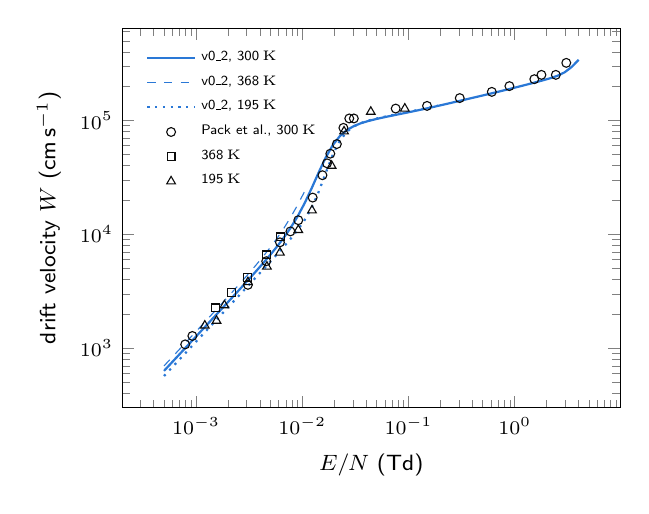
\begin{tikzpicture}
\begin{axis}[width=7.9cm, height=6.4cm, xmode=log, ymode=log,
  xlabel={$E/N$ (Td)}, ylabel={drift velocity $W$ (cm\,s$^{-1}$)},
  tick label style={font=\scriptsize}, label style={font=\footnotesize},
  legend style={font=\tiny, draw=none, fill=none, at={(0.03,0.97)},
  anchor=north west}, legend cell align=left]
\plotcoords{cE, thick}{\wgSwWamodel}
\addlegendentry{v0\_2, 300\unit{K}}
\plotcoords{cE, dashed}{\wgSwWbmodel}
\addlegendentry{v0\_2, 368\unit{K}}
\plotcoords{cE, dotted, thick}{\wgSwWcmodel}
\addlegendentry{v0\_2, 195\unit{K}}
\plotcoords{only marks, mark=o, mark size=1.6pt, ink}{\wgSwWadata}
\addlegendentry{Pack et al., 300\unit{K}}
\plotcoords{only marks, mark=square, mark size=1.4pt, ink}{\wgSwWbdata}
\addlegendentry{368\unit{K}}
\plotcoords{only marks, mark=triangle, mark size=1.8pt, ink}{\wgSwWcdata}
\addlegendentry{195\unit{K}}
\end{axis}
\end{tikzpicture}\hfill
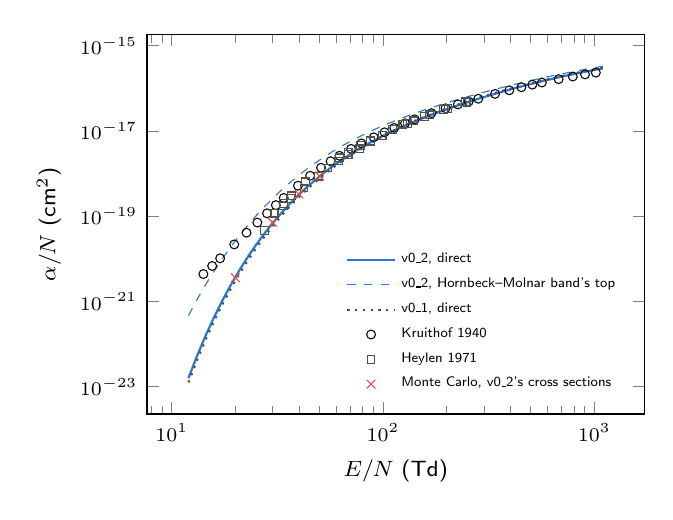
\begin{tikzpicture}
\begin{axis}[width=7.9cm, height=6.4cm, xmode=log, ymode=log,
  xlabel={$E/N$ (Td)}, ylabel={$\alpha/N$ (cm$^2$)},
  tick label style={font=\scriptsize}, label style={font=\footnotesize},
  legend style={font=\tiny, draw=none, fill=none, at={(0.97,0.03)},
  anchor=south east}, legend cell align=left]
\plotcoords{cE, thick}{\wgSwAmodel}
\addlegendentry{v0\_2, direct}
\plotcoords{cE, dashed}{\wgSwAHMmodel}
\addlegendentry{v0\_2, Hornbeck--Molnar band's top}
\plotcoords{ink2, dotted, thick}{\wgSwAoldmodel}
\addlegendentry{v0\_1, direct}
\plotcoords{only marks, mark=o, mark size=1.6pt, ink}{\wgSwAKdata}
\addlegendentry{Kruithof 1940}
\plotcoords{only marks, mark=square, mark size=1.4pt, ink2}{\wgSwAHdata}
\addlegendentry{Heylen 1971}
\plotcoords{only marks, mark=x, mark size=2.2pt, cH}{\wgSwAMCdata}
\addlegendentry{Monte Carlo, v0\_2's cross sections}
\end{axis}
\end{tikzpicture}
\caption{Pure krypton's drift velocity (left) and first Townsend
coefficient (right): v0\_2's two-term solution on Biagi's level-resolved
cross sections against the measurements as Dutton's survey prints
them~\cite{dutton75}. Right: direct ionization (solid), the
Hornbeck--Molnar band's top (dashed), v0\_1 on Biagi's four groups
(dotted) and a Monte Carlo solution of v0\_2's cross
sections~\cite{dias23} (crosses).}
\label{fig:swarm}
\end{figure}

\begin{itemize}
\item \textbf{The drift velocity} of Pack, Voshall and
Phelps~\cite{pack62}, \wg{sw.W.n} points at 195, 300 and 368\unit{K}: rms
\wg{sw.W.rms}\,\% (v0\_1, \wg{sw1.W.rms}\,\%), mean \wg{sw.W.mean}\,\%. It
is \wg{sw.W.r0.rms}\,\% rms below 0.01\unit{Td}, where the electrons are
thermal. Over the runaway from the Ramsauer minimum, 0.01 to
0.05\unit{Td}, it is \wg{sw.W.r1.rms}\,\%: there $W$ rises
\wg{sw.W.r1.wx}-fold while $E/N$ rises \wg{sw.W.r1.ex}-fold. From 0.05 to
3\unit{Td} it is \wg{sw.W.r2.rms}\,\% (mean \wg{sw.W.r2.mean}\,\%). The
largest deviation is \wg{sw.W.worst}\,\% at \wg{sw.W.worst.en}\unit{Td}.
\item \textbf{The ionization coefficient} of Kruithof~\cite{kruithof40} and
Heylen~\cite{heylen71}, \wg{sw.a.n} points to 1017\unit{Td}
(Table~\ref{tab:alpha}). It is \wg{sw.a.r2.rms}\,\% rms from 100 to
300\unit{Td} and \wg{sw.a.r3.mean}\,\% on average above. There the mean
energy passes \wg{sw.a.r3.eps}\unit{eV}, where the two-term approximation
and the steady-state Townsend geometry part ways. From 50 to
100\unit{Td} it is \wg{sw.a.r1.mean}\,\% on average. Below 50\unit{Td} it
is \wg{sw.a.r0.mean}\,\%: \wg{sw.a.r0.K}\,\% against Kruithof and
\wg{sw.a.r0.H}\,\% against Heylen, whose values fall increasingly below
Kruithof's as $E/N$ decreases. At \wg{sw.a.lo.en}\unit{Td} the model is
\x{\wg{sw.a.lo.x}} Kruithof's.
\end{itemize}

\begin{table}[H]
\centering\footnotesize
\begin{tabular}{@{}lrrrr@{}}
\toprule
$E/N$ (Td) & 14 to 50 & 50 to 100 & 100 to 300 & 300 to 1017\\
\midrule
points & \wg{sw.a.r0.n} & \wg{sw.a.r1.n} & \wg{sw.a.r2.n} & \wg{sw.a.r3.n}\\
v0\_1, direct, mean & \wg{sw1.a.r0.mean} & \wg{sw1.a.r1.mean} & \wg{sw1.a.r2.mean} & \wg{sw1.a.r3.mean}\\
v0\_2, direct, mean & \wg{sw.a.r0.mean} & \wg{sw.a.r1.mean} & \wg{sw.a.r2.mean} & \wg{sw.a.r3.mean}\\
\quad against Kruithof, Heylen & \wg{sw.a.r0.K}, \wg{sw.a.r0.H} & \wg{sw.a.r1.K}, \wg{sw.a.r1.H} & \wg{sw.a.r2.K}, \wg{sw.a.r2.H} & \wg{sw.a.r3.K}, \wg{sw.a.r3.H}\\
v0\_2, Hornbeck--Molnar band's top, mean & \wg{swhm.a.r0.mean} & \wg{swhm.a.r1.mean} & \wg{swhm.a.r2.mean} & \wg{swhm.a.r3.mean}\\
\quad against Kruithof, Heylen & \wg{swhm.a.r0.K}, \wg{swhm.a.r0.H} & \wg{swhm.a.r1.K}, \wg{swhm.a.r1.H} & \wg{swhm.a.r2.K}, \wg{swhm.a.r2.H} & \wg{swhm.a.r3.K}, \wg{swhm.a.r3.H}\\
\bottomrule
\end{tabular}
\caption{The ionization coefficient's error (percent, the model less the
measurement over the measurement, averaged over each range's points)
against Kruithof's and Heylen's measurements~\cite{kruithof40,heylen71},
v0\_1 on Biagi's four groups and v0\_2 on his levels, with direct
ionization alone and with every excitation of the levels at or above
\Krtp's energy ionizing associatively.}
\label{tab:alpha}
\end{table}

\textbf{Why v0\_2 falls short below 50\unit{Td}.}
\begin{itemize}
\item \textbf{Not the solver.} LoKI-MC, a Monte Carlo solver with no
two-term approximation~\cite{dias23}, run on v0\_2's own cross sections,
gives an ionization coefficient that v0\_2's two-term solution matches to
\wg{mc.list}\,\% at 20, 30, 40 and 50\unit{Td}. These differences are
within the Monte Carlo's counting error (\wg{mc.stat20}\,\% at
20\unit{Td}, \wg{mc.stat50}\,\% at 50\unit{Td}) and a few percent of the
two-term approximation. The mean energies agree to \wg{mc.mean.max}\,\%.
Bordage et al.\ found the two-term coefficient accurate in krypton against
Monte Carlo too~\cite{bordage13}.
\item \textbf{Not chiefly the cross sections.} Bordage et al.\ compared
every published set of krypton cross sections, and every one gives
coefficients below the measurements at low $E/N$. They call it a general
trend, and ascribe it to the measurements' contribution from Penning
ionization of impurities, which grows as $E/N$ falls~\cite{bordage13}.
Resolving Biagi's four groups into his \wg{par.levels} levels moves the
mean below 50\unit{Td} from \wg{sw1.a.r0.mean} to \wg{sw.a.r0.mean}\,\%.
\item \textbf{The measurements disagree.} Heylen's values fall up to
\x{\wg{kh.max}} below Kruithof's near 30\unit{Td}, and Jacques et al.\ also found
values below Kruithof's at the low end of their range in
krypton~\cite{jacques86}.
\item \textbf{One process of pure krypton.} An atom excited at or above
\wg{hm.eai}\unit{eV}, the energy of \Krtp{} relative to two ground-state
atoms~\cite{ng77}, can ionize on a ground-state atom. Hornbeck and Molnar
found \Krtp{} made by electrons \wg{hm.ap}\unit{V} below the energy that
makes \Krp, and traced it to that collision~\cite{hornbeck51}. The
electrons' distribution falls by orders of magnitude between those
levels and the \wm{E.ion}-eV threshold, so at its top the band raises the
coefficient \x{\wg{hm.x14}} at 14\unit{Td}, \x{\wg{hm.x30}} at
30\unit{Td} and \x{\wg{hm.x100}} at 100\unit{Td}. At its top
\wg{hm.inside} of the \wg{hm.n} points below 50\unit{Td} lie between the
band's two ends, and the \wg{hm.above} of Kruithof's at and below
\wg{hm.above.en}\unit{Td} lie above even its top, which reaches
\wg{hm.above.lo} to \wg{hm.above.hi} of them. The same top makes the
model's mean error from 100 to 300\unit{Td} \wg{swhm.a.r2.mean}\,\%,
where direct ionization alone is within \wg{sw.a.r2.rms}\,\% rms
(Table~\ref{tab:alpha}). So a share near 1
cannot hold at every field. It need not: the share is how fast the
excited atom meets a partner against how fast it radiates or is quenched,
so it grows with the pressure; and a Townsend experiment needs a larger
pressure times gap where the coefficient is small, so its low-field
points come from higher pressures. The pressures of these measurements
are not in Dutton's tables,
and no measurement in hand gives the share for krypton, so the band
cannot be scored here. It stays at 0 by default, as every unmeasured row
does.
\end{itemize}

\textbf{What this means for the reference point.} The electrons sit at
\wg{ref.kin.en.lo} to \wg{ref.kin.en.hi}\unit{Td}, where the low
ionization coefficient would apply. There direct ionization makes
\wm{ion.C2}\,\% of the ions and Penning ionization the rest, so this
error does not reach the answer: the Hornbeck--Molnar band at its top
moves the 147-nm share by \wg{unc.hm.cut}\,\%. It would matter where
direct ionization does. No swarm measurement scores the excitation
rates, which do decide the answer.

\section{Under an electron beam}
\label{sec:beam}

Three measurements bear on the chain from excitation to the 147-nm
photon. They were made under electron beams, so for them v0\_2 runs under
a beam drive. The drive is a fixture of this note, not part of the model.
It deposits the given power as ion pairs, \Krs, \Krpp{} and secondary
electrons in the proportions of a fast electron's degradation in pure
krypton. That degradation is the Fowler--Spencer--Fano recursion on the
same Biagi cross sections, level by level, from \wg{beam.e0}\unit{eV}: an excitation
continues the electron at $E-I$, and an ionization shares $E-I$ equally
between the two electrons. Per ion pair it gives:
\begin{itemize}
\item $W=\wg{beam.W}\unit{eV}$;
\item \wg{beam.pp} \Krpp, from the levels above the 5s manifold;
\item \wg{beam.s} \Krs, from the four 5s levels;
\item \wg{beam.cascade}\unit{eV} of heat, the levels' excess over the
energy of the species they make;
\item \wg{beam.eps}\unit{eV} of sub-excitation secondaries, which the
kinetic equation injects with a flat spectrum up to \wm{E.S}\unit{eV}.
\end{itemize}
That is one excitation or ion per \wg{beam.ws}\unit{eV}.

\textbf{The partition.} Saito et al.~\cite{saito03} measured scintillation
photons and electrons together under 5.49-MeV alpha particles in 1 to
10\unit{atm} of krypton. They found \wg{saito.nex} excited atoms per ion pair, and
$W_s=\wg{saito.ws}\unit{eV}$, the energy per photon when every pair
recombines.
They also confirmed that each recombination gives one photon. The drive's
\wg{beam.ws}\unit{eV} per excitation or ion is \wg{beam.ws.dev}\,\% from
their $W_s$. Its excitations per pair (\wg{beam.nex}) differ from theirs
by \wg{beam.nex.dev}\,\%, and its $W$ differs by \wg{beam.W.dev}\,\% from
the \wg{saito.W}\unit{eV} their two numbers imply. The two errors cancel
in the quantity the light depends on. One photon of \wg{hv147}\unit{eV}
per \wg{saito.ws}\unit{eV} is an efficiency of \wg{saito.ideal}. v0\_2's
ceiling, one photon per excitation and per ion of the drive, is
\wg{beam.ceil}.

\textbf{Low pump.} Morozov et al.~\cite{morozov08} measured the power a
continuous 8 to 15-keV beam deposits in the gas against the VUV power
emitted into $4\pi$. For krypton they found \wg{moz.meas} $\pm$ \wg{moz.err}, flat from 500
to 1400\unit{hPa} and over a tenfold range of beam power. At
\wg{moz.hpa}\unit{hPa}, \wg{moz.w.lo} and \wg{moz.w.hi}\unit{W\,cm^{-3}}
for \wg{beam.pulse}\unit{\mu s} with the light counted for
\wg{beam.tail.lo}\unit{\mu s} after, v0\_2 gives \wg{moz.30.kin} and
\wg{moz.300.kin} (Table~\ref{tab:beam}). The error is \wg{moz.kin.dev}\,\%,
\wg{moz.kin.sig} of the measurement's standard errors. At this pump
nothing competes with the light: \wg{moz.300.kin.G2} Penning ionizations
per pair, every ion recombined (\wg{moz.300.kin.rec} per pair), and every
\Krts{} radiating. So v0\_2 sits at its ceiling, which Saito et al.'s
measurement supports. Morozov et al.\ compare their value with calculated
maxima of 0.46 and 0.52 for krypton. The \wg{moz.short}\,\% between their
value and Saito et al.'s one photon per excitation and per ion
(\wg{saito.ideal}) is not explained in v0\_2.

\textbf{High pump.} Eckstrom et al.~\cite{eckstrom88} report the
fluorescence efficiency of \Krts{} near their theoretical limit of about
46\,\%. They found it under a low-current, long-pulse beam at modest
pressures, for pump rates up to $3\times10^5\unit{W\,cm^{-3}}$. The
abstract does not give the pressure of each point. At that pump rate
(1\unit{\mu s}, the light counted for \wg{beam.tail.hi}\unit{\mu s})
v0\_2 gives:
\begin{itemize}
\item \wg{eck.0.5.kin} at 0.5\unit{atm}, \wg{eck.1.kin} at 1\unit{atm}
and \wg{eck.2.kin} at 2\unit{atm}, that is \wg{eck.0.5.kin.loss},
\wg{eck.1.kin.loss} and \wg{eck.2.kin.loss}\,\% below its ceiling of
\wg{beam.ceil};
\item at 1\unit{atm}, Penning ionization of \Krs{} by \Krs{} costs
\wg{eck.1.kin.G2} photons per pair, because the excimer forms too slowly to
outrun it;
\item at 1\unit{atm} with \Krs{} + \Krs{} at its band's low end,
\wg{eck_pen.1.kin} (\wg{eck_pen.1.kin.loss}\,\% below the ceiling), and
with \Krs{} + 2Kr at its band's top, \wg{eck_form.1.kin}
(\wg{eck_form.1.kin.loss}\,\%).
\end{itemize}
Their limit assumes other numbers than v0\_2's ceiling, so what the
report tests is the loss: little at high pump. v0\_2 loses little at
2\unit{atm}. If their pressures were near 1\unit{atm}, the report leans
toward a weaker Penning loss or a faster formation than the defaults.
Those are the two inputs that also lead the field-driven uncertainty.

\begin{table}[H]
\centering\footnotesize
\resizebox{\linewidth}{!}{%
\begin{tabular}{@{}llrrrrrr@{}}
\toprule
run & measured & kinetic & two-temperature & Penning per pair & photons per pair & $T_e$ (eV) & $T_g$ end (K)\\
\midrule
\wg{moz.w.lo}\unit{W\,cm^{-3}}, \wg{moz.hpa}\unit{hPa} & \wg{moz.meas} $\pm$ \wg{moz.err} & \wg{moz.30.kin} & \wg{moz.30.2t} & \wg{moz.30.kin.G2} & \wg{moz.30.kin.ph} & \wg{moz.30.kin.te} & \wg{moz.30.kin.tg}\\
\wg{moz.w.hi}\unit{W\,cm^{-3}}, \wg{moz.hpa}\unit{hPa} & \wg{moz.meas} $\pm$ \wg{moz.err} & \wg{moz.300.kin} & \wg{moz.300.2t} & \wg{moz.300.kin.G2} & \wg{moz.300.kin.ph} & \wg{moz.300.kin.te} & \wg{moz.300.kin.tg}\\
$3\times10^5\unit{W\,cm^{-3}}$, 0.5\unit{atm} & near \wg{eck.meas} & \wg{eck.0.5.kin} & \wg{eck.0.5.2t} & \wg{eck.0.5.kin.G2} & \wg{eck.0.5.kin.ph} & \wg{eck.0.5.kin.te} & \wg{eck.0.5.kin.tg}\\
$3\times10^5\unit{W\,cm^{-3}}$, 1\unit{atm} & near \wg{eck.meas} & \wg{eck.1.kin} & \wg{eck.1.2t} & \wg{eck.1.kin.G2} & \wg{eck.1.kin.ph} & \wg{eck.1.kin.te} & \wg{eck.1.kin.tg}\\
$3\times10^5\unit{W\,cm^{-3}}$, 2\unit{atm} & near \wg{eck.meas} & \wg{eck.2.kin} & \wg{eck.2.2t} & \wg{eck.2.kin.G2} & \wg{eck.2.kin.ph} & \wg{eck.2.kin.te} & \wg{eck.2.kin.tg}\\
\quad 1\unit{atm}, \Krs{} + \Krs{} $\wm{bd.kr_pen.lo}$ & & \wg{eck_pen.1.kin} & \wg{eck_pen.1.2t} & \wg{eck_pen.1.kin.G2} & \wg{eck_pen.1.kin.ph} & \wg{eck_pen.1.kin.te} & \wg{eck_pen.1.kin.tg}\\
\quad 1\unit{atm}, \Krs{} + 2Kr $\wm{bd.kr2_form.hi}$ & & \wg{eck_form.1.kin} & \wg{eck_form.1.2t} & \wg{eck_form.1.kin.G2} & \wg{eck_form.1.kin.ph} & \wg{eck_form.1.kin.te} & \wg{eck_form.1.kin.tg}\\
\bottomrule
\end{tabular}}
\caption{v0\_2 under the beam drive: the VUV efficiency (147-nm energy
over the deposited energy) on both closures, and on the kinetic EEDF the
Penning ionizations and 147-nm photons per ion pair, the pulse's mean
$T_e$ and the final gas temperature. v0\_2's ceiling, one photon per
excitation and per ion, is \wg{beam.php} photons per pair, an efficiency
of \wg{beam.ceil}; Saito et al.'s ideal is \wg{saito.ideal}.}
\label{tab:beam}
\end{table}

\section{The energy ladder}

Figure~\ref{fig:ladder} draws v0\_2's levels at their formation energies
and the rows that move energy between them.

\begin{figure}[H]
\centering
\begin{tikzpicture}[x=1cm, y=0.6cm, font=\scriptsize,
  arr/.style={-{Stealth[length=4pt]}},
  heat/.style={cH, decorate, decoration={snake, amplitude=1pt,
    segment length=4pt, post length=4pt}, -{Stealth[length=4pt]}}]
\newcommand\lev[4]{\draw[line width=1.1pt, #4] (#1,#3) -- (#2,#3);}
% atoms
\lev{0}{4.6}{0}{ink}
\lev{0}{4.6}{\wg{lad.S}}{cX}
\lev{0}{4.6}{\wg{lad.P}}{cP}
\lev{0}{4.6}{\wg{lad.I}}{cI}
\node[left] at (0,0) {Kr, 0};
\node[left] at (0,\wg{lad.S}) {\Krs{} (5s) \wg{lad.S}};
\node[left] at (0,\wg{lad.P}) {\Krpp{} (5p) \wg{lad.P}};
\node[left] at (0,\wg{lad.I}) {\Krp{} \wg{lad.I}};
% molecules
\lev{7.4}{9.6}{0}{ink}
\lev{7.4}{9.6}{\wg{lad.X2}}{cV}
\lev{7.4}{9.6}{\wg{lad.I2}}{cI}
\draw[ink2, dashed] (7.4,\wg{lad.low}) -- (9.6,\wg{lad.low});
\node[right] at (9.6,0) {2Kr, 0};
\node[right] at (9.6,\wg{lad.X2}) {\Krts{} \wg{lad.X2}};
\node[right] at (9.6,\wg{lad.I2}) {\Krtp{} \wg{lad.I2}};
\node[right, ink2] at (9.6,\wg{lad.low}) {repulsive 2Kr, \wg{lad.low}};
% electron impact from the ground state
\draw[cE, arr] (0.4,0) -- (0.4,\wg{lad.S}) node[pos=0.45, right] {G1};
\draw[cE, arr] (1.0,0) -- (1.0,\wg{lad.P}) node[pos=0.45, right] {C1};
\draw[cE, arr] (1.6,0) -- (1.6,\wg{lad.I}) node[pos=0.45, right] {C2};
% Penning ionization of Kr* by Kr*
\draw[ink2, densely dashed, arr] (2.3,\wg{lad.S}) -- (2.3,\wg{lad.I})
  node[pos=0.75, right] {G2};
% the 5s <-> 5p cycle, its relaxation and its light
\draw[cE, arr] (3.0,\wg{lad.S}) -- (3.0,\wg{lad.P});
\draw[cE, arr] (3.25,\wg{lad.P}) -- (3.25,\wg{lad.S});
\draw[heat] (3.75,\wg{lad.P}) -- (3.75,\wg{lad.S});
\draw[cP, arr] (4.25,\wg{lad.P}) -- (4.25,\wg{lad.S});
\node[ink, anchor=north west, align=left, inner sep=1pt] at (2.75,9.6)
  {\textcolor{cE}{K76, K76r,}\\ \textcolor{cH}{KPS},
  \textcolor{cP}{PRAD}};
% to the excimer and its light
\draw[cX, arr] (4.6,\wg{lad.S}) -- (7.4,\wg{lad.X2});
\node[cX, anchor=north west] at (4.7,9.15) {AK8\_Kr, \wg{lad.ak8} to heat};
\draw[cV, arr] (8.1,\wg{lad.X2}) -- (8.1,\wg{lad.low})
  node[pos=0.5, right, cV] {KR2\_RAD, $h\nu$ \wg{lad.hv}};
\draw[heat] (8.1,\wg{lad.low}) -- (8.1,0);
% the ions
\draw[cI, arr] (4.6,\wg{lad.I}) -- (7.4,\wg{lad.I2});
\node[cI, anchor=south west] at (7.45,13.25) {K15, \wg{lad.k15} to heat};
\draw[cI, arr] (7.4,\wg{lad.I2}) -- (4.6,\wg{lad.P});
\node[cI, anchor=north west] at (7.45,12.4) {R11p, \wg{lad.r11} to heat};
\end{tikzpicture}
\caption{v0\_2's energy ladder in eV above ground-state krypton at rest.
A bar is a species at its formation energy. Blue arrows are electron
impact, which takes its energy from the electron gas; K76r, the 5p
\ra 5s arrow beside K76, returns it. The dashed G2 is \Krs{} + \Krs{}
\ra \Krp{} + Kr + \el, which gives \wg{lad.pen}\unit{eV} to the electron.
A red squiggle is heat: KPS relaxes the 5p rung on krypton, and PRAD
radiates the \wg{lad.gap}-eV gap in the near infrared. The
excimer radiates onto the repulsive ground state, which falls apart and
heats the gas. G1's four 5s levels, \wg{lad.s1} to \wg{lad.s2}\unit{eV},
make \Krs; C1's levels, \wg{lad.c1lo} to \wg{lad.c1hi}\unit{eV}, cascade
to the 5p rung; each heats the gas with its excess. HM, the
Hornbeck--Molnar ionization of the levels above \Krtp's energy, is a band
at 0 and not drawn.}
\label{fig:ladder}
\end{figure}

\section{Where v0\_2 is not yet reliable}

\begin{itemize}
\item \textbf{\Krs{} + 2Kr.} The excimer's formation rate is the largest
term of the propagated uncertainty: its measurements spread by a factor
of \wg{form.ratio}. Its temperature law is measured to 451\unit{K}, and
the reference point ends at \wg{ref.kin.tg}\unit{K}.
\item \textbf{The field-driven regime is unscored.} No pure-krypton
measurement in hand tests the 5s $\leftrightarrow$ 5p cycle under a field.
Its cross sections are measured to $\pm$\wg{jung.unc.1s5} to
\wg{jung.unc.1s3}\,\%. Those of the two $J=1$ levels are not measured;
they are the band's low end.
\item \textbf{The rows with no measurement.} \Krts{} + \Krts{} and the
stepwise ionizations of \Krs{} and \Krpp{} are 0 by default. Each at its
band's top cuts the 147-nm share by a fifth to a half
(Table~\ref{tab:unc}).
\item \textbf{\Krs{} + \Krs.} Its $\wm{k.G2}\cm{3}$ is a 1974
measurement~\cite{leichner74} as Kannari et al.\ print it~\cite{kannari85}.
The e-beam report at high pump leans toward a lower value
(Section~\ref{sec:beam}).
\item \textbf{The e-beam efficiency at low pump} is off Morozov et
al.'s by \wg{moz.kin.dev}\,\%, and v0\_2 holds no process that would
explain the difference.
\item \textbf{The ionization coefficient below 50\unit{Td}} has a mean
error of \wg{sw.a.r0.mean}\,\%, as every published cross-section set
falls below these measurements~\cite{bordage13}. This does not reach the
reference point, where Penning ionization makes the ions.
\item \textbf{The Hornbeck--Molnar share} of the levels above
\wg{hm.eai}\unit{eV} is not measured for krypton and is 0 by default. At
its top it brackets most of the low-field measurements, overshoots those
from 100 to 300\unit{Td} (\wg{swhm.a.r2.mean}\,\%) and moves the
reference point by \wg{unc.hm.cut}\,\%.
\item \textbf{Processes v0\_2 does not carry}, each needing a measured rate
before it can enter:
\begin{itemize}
\item Kr$_3^+$ and its recombination;
\item electron collisions with \Krts{}: ionization, quenching and the
mixing of its two states (v0\_2 carries one state at the slow component's
270\unit{ns});
\item Penning ionization between \Krs{} and \Krts, and of \Krpp;
\item the redissociation of \Krtp{} and \Krts{} in hot gas;
\item the resonance lines of the two $J=1$ 5s levels.
\end{itemize}
Three-body recombination \Krp{} + \el{} + \el~\cite{mansbach69} is not
carried either: at 1\unit{atm} \Krp{} converts to \Krtp{} in
\wg{k15.ns}\unit{ns}.
\item \textbf{The kinetic EEDF's steady shape.} Between renewals the EEDF
keeps its steady shape, which the first nanosecond and the afterglow
strain. The two-temperature closure reads a tail table made for LIGHT's
Kr/F$_2$ network on Biagi's four groups (its F$_2=0$ column); the default
closure does not use it.
\end{itemize}

\textbf{How the numbers were made.} Every number in this note is computed
from the model when the note is built. None is
typed by hand except the measurements, which carry their sources. The
runs are cached under a hash of the model's code, so a change to the
model reruns them all (code \texttt{\wg{md5}}). The kinetic runs take
about \wg{ref.kin.min} minutes each; the two-temperature runs take
seconds.

\clearpage
\appendix
\section{Reaction rates}
\label{app:rates}

The rows of v0\_2 with the values they run with and their sources.
Electron-impact rows use their cross sections over the kinetic EEDF (or
the two-temperature closure). A band gives its default and its two ends.

\begin{table}[H]
\centering\scriptsize
\renewcommand{\arraystretch}{1.12}
\begin{tabularx}{\linewidth}{@{}>{\raggedright\arraybackslash}p{1.35cm}>{\raggedright\arraybackslash}p{3.6cm}>{\raggedright\arraybackslash}p{4.1cm}>{\raggedright\arraybackslash}X@{}}
\toprule
row & reaction & value & source\\
\midrule
G1 & \el{} + Kr \ra \el{} + \Krs(5s) & the four 5s levels, \wm{E.S} to \wg{lad.s2}\unit{eV}, each at its threshold; the excess over \wm{E.S} to heat & Biagi, Magboltz 8.97~\cite{biagi99,pancheshnyi12,carbone21}\\
C1 & \el{} + Kr \ra \el{} + \Krpp & the 5p, 4d, 6s and higher levels, \wg{lad.c1lo} to \wg{lad.c1hi}\unit{eV}, each at its threshold; the excess over \wm{E.PP} to heat & Biagi, Magboltz 8.97\\
HM & \el{} + Kr (+ Kr) \ra \Krtp{} + 2\el & the share of the excitations of the \wg{hm.levels} levels at or above \wg{hm.eai}\unit{eV}; band 0 (default) to 1 & no measurement for krypton; the process, Hornbeck and Molnar~\cite{hornbeck51}\\
C2 & \el{} + Kr \ra \Krp{} + 2\el & \wm{E.ion}\unit{eV} & Biagi, Magboltz 8.97\\
G6 & \el{} + Kr, elastic & the momentum transfer cross section & Biagi, Magboltz 8.97\\
K76 & \el{} + \Krs{} \ra \el{} + \Krpp & the lumped measured cross section, $\wg{jung.sig6}\unit{cm^2}$ at 6\unit{eV}; band \x{} \wm{bd.k_5s5p.lo} to \wm{bd.k_5s5p.hi} & Jung et al.~\cite{jung06,jung05}; Kannari's fit as a comparison~\cite{kannari85,jacob76}\\
K76r & \el{} + \Krpp{} \ra \el{} + \Krs & detailed balance, $g$ 12/36 over the \wm{gap5p}-eV gap & \\
KPS & \Krpp{} + Kr \ra \Krs{} + Kr & $\wm{k.KPS}\cm{3}$; band $\wm{bd.kps_kr.lo}$ to the default & Gazeli et al.~\cite{gazeli21}, one level, products unresolved; the low end lies in the range Chang and Setser measured for argon's 4p levels in argon, $2\times10^{-11}$ to $10^{-10}$~\cite{chang78}\\
PRAD & \Krpp{} \ra \Krs{} + $h\nu$, 760--830\unit{nm} & $\tau=\wg{tau5p}\unit{ns}$, the $2J+1$ mean of the ten 5p levels & Dzier\.z\k{e}ga et al.~\cite{dzierzega00}; a TALIF lifetime of one level, 34.1\unit{ns}, as a cross-check~\cite{gazeli21rev}\\
G2 & \Krs{} + \Krs{} \ra \Krp{} + Kr + \el & $\wm{k.G2}\cm{3}$; band $\wm{bd.kr_pen.lo}$ to the default & Leichner and Ericson~\cite{leichner74} as Kannari et al.\ print it~\cite{kannari85}; the low end has no published measurement\\
AK8\_Kr & \Krs{} + 2Kr \ra \Krts{} + Kr & $\wm{k.AK8}\cm{6}\times(T_g/300)^{\wm{tpow.AK8}}$; band to $\wm{bd.kr2_form.hi}$ & Ueda et al.\ at 0.5--1\unit{atm}~\cite{ueda84}; afterglows~\cite{salamero79,tracy76,smith63} and Hughes's value~\cite{quigley78} inside the band; the law, Wieme and Lenaerts~\cite{wieme81}\\
KR2\_RAD & \Krts{} \ra 2Kr + $h\nu$, 147\unit{nm} & $\tau=\wm{tauRAD}\unit{ns}$, $h\nu=\wm{hv.RAD}\unit{eV}$ & Morikawa et al., 270 $\pm$ 5\unit{ns}~\cite{morikawa89}; 250 $\pm$ 20~\cite{salamero79}, 280 $\pm$ 30~\cite{quigley78}\\
PEN\_KR2 & \Krts{} + \Krts{} \ra \Krtp{} + 2Kr + \el & 0; band to $\wm{bd.kr2_pen.hi}$ & no measurement; Kannari et al.'s value is the top~\cite{kannari85}\\
K15 & \Krp{} + 2Kr \ra \Krtp{} + Kr & $\wm{k.K15}\cm{6}\times(T_g/300)^{\wm{tpow.K15}}$ & the mean of three measurements~\cite{bhattacharya70,grossl81,smith72}; the law, P\'erez-R\'ios and Greene~\cite{perezrios18}\\
R11p & \Krtp{} + \el{} \ra \Krpp{} + Kr & $\wm{k.R11p}\,(300\,\mathrm{K}/T_e)^{\wm{pow.R11p}}\cm{3}$, $\pm$10\,\% & Shiu and Biondi~\cite{shiu77}; Mikus within 8\,\%~\cite{mikus78}\\
KSTEP\_S & \el{} + \Krs{} \ra \Krp{} + 2\el & 0; band to $\wm{bd.kstep_s.hi}\,T_e^{0.68}e^{-4.04/T_e}\cm{3}$ & no measurement; Vriens' calculation~\cite{vriens65} as Kannari et al.\ print it~\cite{kannari85}\\
KSTEP\_P & \el{} + \Krpp{} \ra \Krp{} + 2\el & 0; band to $\wm{bd.kstep_p.hi}\,T_e^{0.62}e^{-2.53/T_e}\cm{3}$ & the same\\
\bottomrule
\end{tabularx}
\caption{v0\_2's rows. Rates in cm$^3$\,s$^{-1}$ or cm$^6$\,s$^{-1}$, $T_e$
in eV. Two rows sit in the optional group \texttt{electron}, off by
default: a stepwise-ionization template of \Krs{} and the superelastic
return of the 5s levels by detailed balance. \Krtp{} lies \wg{lad.k15}\unit{eV} below \Krp{}
+ Kr~\cite{ng77}; \Krts{}'s \wg{lad.ak8}-eV well is an estimate that moves
energy only between storage and heat.}
\end{table}

\begin{thebibliography}{99}
\footnotesize
\setlength{\itemsep}{1pt}
\bibitem{biagi99} S.~F.~Biagi, Nucl.\ Instrum.\ Methods A 421, 234 (1999), doi:10.1016/S0168-9002(98)01233-9.
\bibitem{bordage13} M.~C.~Bordage, S.~F.~Biagi, L.~L.~Alves, K.~Bartschat, S.~Chowdhury, L.~C.~Pitchford, G.~J.~M.~Hagelaar, W.~L.~Morgan, V.~Puech and O.~Zatsarinny, J.\ Phys.\ D 46, 334003 (2013), doi:10.1088/0022-3727/46/33/334003.
\bibitem{dias23} T.~C.~Dias, A.~Tejero-del-Caz, L.~L.~Alves and V.~Guerra, Comput.\ Phys.\ Commun.\ 282, 108554 (2023), doi:10.1016/j.cpc.2022.108554.
\bibitem{hornbeck51} J.~A.~Hornbeck and J.~P.~Molnar, Phys.\ Rev.\ 84, 621 (1951), doi:10.1103/PhysRev.84.621.
\bibitem{jacques86} L.~Jacques, W.~Bruynooghe, R.~Boucique and W.~Wieme, J.\ Phys.\ D 19, 1731 (1986), doi:10.1088/0022-3727/19/9/017.
\bibitem{pancheshnyi12} S.~Pancheshnyi et al., Chem.\ Phys.\ 398, 148 (2012), doi:10.1016/j.chemphys.2011.04.020.
\bibitem{carbone21} E.~Carbone et al., Atoms 9, 16 (2021), doi:10.3390/atoms9010016.
\bibitem{hagelaar05} G.~J.~M.~Hagelaar and L.~C.~Pitchford, Plasma Sources Sci.\ Technol.\ 14, 722 (2005), doi:10.1088/0963-0252/14/4/011.
\bibitem{jung05} R.~O.~Jung, T.~E.~Stone, J.~B.~Boffard, L.~W.~Anderson and C.~C.~Lin, Phys.\ Rev.\ Lett.\ 94, 163202 (2005), doi:10.1103/PhysRevLett.94.163202.
\bibitem{jung06} R.~O.~Jung, T.~E.~Stone, J.~B.~Boffard, L.~W.~Anderson and C.~C.~Lin, Phys.\ Rev.\ A 73, 022722 (2006), doi:10.1103/PhysRevA.73.022722.
\bibitem{kannari85} F.~Kannari, M.~Obara and T.~Fujioka, J.\ Appl.\ Phys.\ 57, 4309 (1985), doi:10.1063/1.334590.
\bibitem{jacob76} J.~H.~Jacob and J.~A.~Mangano, Appl.\ Phys.\ Lett.\ 28, 724 (1976), doi:10.1063/1.88629.
\bibitem{vriens65} L.~Vriens, Physica 31, 385 (1965), doi:10.1016/0031-8914(65)90043-1.
\bibitem{gazeli21} K.~Gazeli et al., Phys.\ Plasmas 28, 043301 (2021), doi:10.1063/5.0041471.
\bibitem{gazeli21rev} K.~Gazeli, G.~Lombardi, X.~Aubert, C.~Y.~Duluard, S.~Prasanna and K.~Hassouni, Plasma 4, 145 (2021), doi:10.3390/plasma4010009.
\bibitem{chang78} R.~S.~F.~Chang and D.~W.~Setser, J.\ Chem.\ Phys.\ 69, 3885 (1978), doi:10.1063/1.437126.
\bibitem{dzierzega00} K.~Dzier\.z\k{e}ga, U.~Volz, G.~Nave and U.~Griesmann, Phys.\ Rev.\ A 62, 022505 (2000), doi:10.1103/PhysRevA.62.022505.
\bibitem{leichner74} P.~K.~Leichner and R.~J.~Ericson, Phys.\ Rev.\ A 9, 251 (1974), doi:10.1103/PhysRevA.9.251.
\bibitem{ueda84} K.~Ueda, S.~Kanada, A.~Sasaki and H.~Takuma, Rev.\ Laser Eng.\ 12, 357 (1984), doi:10.2184/lsj.12.357.
\bibitem{salamero79} Y.~Salamero et al., J.\ Phys.\ B 12, 419 (1979), doi:10.1088/0022-3700/12/3/019.
\bibitem{tracy76} C.~J.~Tracy and H.~J.~Oskam, J.\ Chem.\ Phys.\ 65, 1666 (1976), doi:10.1063/1.433312.
\bibitem{smith63} D.~S.~Smith and R.~Turner, Can.\ J.\ Phys.\ 41, 1949 (1963), doi:10.1139/p63-195.
\bibitem{quigley78} G.~P.~Quigley and W.~M.~Hughes, Appl.\ Phys.\ Lett.\ 32, 649 (1978), doi:10.1063/1.89882.
\bibitem{wieme81} W.~Wieme and J.~Lenaerts, J.\ Chem.\ Phys.\ 74, 483 (1981), doi:10.1063/1.440855.
\bibitem{morikawa89} E.~Morikawa et al., J.\ Chem.\ Phys.\ 91, 1469 (1989), doi:10.1063/1.457108.
\bibitem{bhattacharya70} A.~K.~Bhattacharya, Phys.\ Rev.\ A 1, 1196 (1970), doi:10.1103/PhysRevA.1.1196.
\bibitem{grossl81} M.~Gr\"ossl et al., J.\ Chem.\ Phys.\ 74, 1728 (1981), doi:10.1063/1.441261.
\bibitem{smith72} D.~Smith, A.~G.~Dean and I.~C.~Plumb, J.\ Phys.\ B 5, 2134 (1972), doi:10.1088/0022-3700/5/11/020.
\bibitem{perezrios18} J.~P\'erez-R\'ios and C.~H.~Greene, Phys.\ Rev.\ A 98, 062707 (2018), doi:10.1103/PhysRevA.98.062707.
\bibitem{shiu77} Y.-J.~Shiu and M.~A.~Biondi, Phys.\ Rev.\ A 16, 1817 (1977), doi:10.1103/PhysRevA.16.1817.
\bibitem{mikus78} O.~Mikus, J.\ Phys.\ D 11, L39 (1978), doi:10.1088/0022-3727/11/3/003.
\bibitem{ng77} C.~Y.~Ng, D.~J.~Trevor, B.~H.~Mahan and Y.~T.~Lee, J.\ Chem.\ Phys.\ 66, 446 (1977), doi:10.1063/1.433989.
\bibitem{mansbach69} P.~Mansbach and J.~Keck, Phys.\ Rev.\ 181, 275 (1969), doi:10.1103/PhysRev.181.275.
\bibitem{pack62} J.~L.~Pack, R.~E.~Voshall and A.~V.~Phelps, Phys.\ Rev.\ 127, 2084 (1962), doi:10.1103/PhysRev.127.2084.
\bibitem{dutton75} J.~Dutton, J.\ Phys.\ Chem.\ Ref.\ Data 4, 577 (1975), doi:10.1063/1.555525, Tables 1.9 and 7.4.
\bibitem{kruithof40} A.~A.~Kruithof, Physica 7, 519 (1940), doi:10.1016/S0031-8914(40)90043-X.
\bibitem{heylen71} A.~E.~D.~Heylen, Int.\ J.\ Electron.\ 31, 19 (1971), doi:10.1080/00207217108938196.
\bibitem{saito03} K.~Saito, S.~Sasaki, H.~Tawara, T.~Sanami and E.~Shibamura, IEEE Trans.\ Nucl.\ Sci.\ 50, 2452 (2003), doi:10.1109/TNS.2003.820615.
\bibitem{morozov08} A.~Morozov, T.~Heindl, R.~Kr\"ucken, A.~Ulrich and J.~Wieser, J.\ Appl.\ Phys.\ 103, 103301 (2008), doi:10.1063/1.2931000.
\bibitem{eckstrom88} D.~J.~Eckstrom et al., J.\ Appl.\ Phys.\ 64, 1691 (1988), doi:10.1063/1.341762.
\end{thebibliography}

\end{document}
